% Options for packages loaded elsewhere
\PassOptionsToPackage{unicode}{hyperref}
\PassOptionsToPackage{hyphens}{url}
\documentclass[
]{book}
\usepackage{xcolor}
\usepackage{amsmath,amssymb}
\setcounter{secnumdepth}{5}
\usepackage{iftex}
\ifPDFTeX
  \usepackage[T1]{fontenc}
  \usepackage[utf8]{inputenc}
  \usepackage{textcomp} % provide euro and other symbols
\else % if luatex or xetex
  \usepackage{unicode-math} % this also loads fontspec
  \defaultfontfeatures{Scale=MatchLowercase}
  \defaultfontfeatures[\rmfamily]{Ligatures=TeX,Scale=1}
\fi
\usepackage{lmodern}
\ifPDFTeX\else
  % xetex/luatex font selection
\fi
% Use upquote if available, for straight quotes in verbatim environments
\IfFileExists{upquote.sty}{\usepackage{upquote}}{}
\IfFileExists{microtype.sty}{% use microtype if available
  \usepackage[]{microtype}
  \UseMicrotypeSet[protrusion]{basicmath} % disable protrusion for tt fonts
}{}
\makeatletter
\@ifundefined{KOMAClassName}{% if non-KOMA class
  \IfFileExists{parskip.sty}{%
    \usepackage{parskip}
  }{% else
    \setlength{\parindent}{0pt}
    \setlength{\parskip}{6pt plus 2pt minus 1pt}}
}{% if KOMA class
  \KOMAoptions{parskip=half}}
\makeatother
\usepackage{color}
\usepackage{fancyvrb}
\newcommand{\VerbBar}{|}
\newcommand{\VERB}{\Verb[commandchars=\\\{\}]}
\DefineVerbatimEnvironment{Highlighting}{Verbatim}{commandchars=\\\{\}}
% Add ',fontsize=\small' for more characters per line
\usepackage{framed}
\definecolor{shadecolor}{RGB}{248,248,248}
\newenvironment{Shaded}{\begin{snugshade}}{\end{snugshade}}
\newcommand{\AlertTok}[1]{\textcolor[rgb]{0.94,0.16,0.16}{#1}}
\newcommand{\AnnotationTok}[1]{\textcolor[rgb]{0.56,0.35,0.01}{\textbf{\textit{#1}}}}
\newcommand{\AttributeTok}[1]{\textcolor[rgb]{0.13,0.29,0.53}{#1}}
\newcommand{\BaseNTok}[1]{\textcolor[rgb]{0.00,0.00,0.81}{#1}}
\newcommand{\BuiltInTok}[1]{#1}
\newcommand{\CharTok}[1]{\textcolor[rgb]{0.31,0.60,0.02}{#1}}
\newcommand{\CommentTok}[1]{\textcolor[rgb]{0.56,0.35,0.01}{\textit{#1}}}
\newcommand{\CommentVarTok}[1]{\textcolor[rgb]{0.56,0.35,0.01}{\textbf{\textit{#1}}}}
\newcommand{\ConstantTok}[1]{\textcolor[rgb]{0.56,0.35,0.01}{#1}}
\newcommand{\ControlFlowTok}[1]{\textcolor[rgb]{0.13,0.29,0.53}{\textbf{#1}}}
\newcommand{\DataTypeTok}[1]{\textcolor[rgb]{0.13,0.29,0.53}{#1}}
\newcommand{\DecValTok}[1]{\textcolor[rgb]{0.00,0.00,0.81}{#1}}
\newcommand{\DocumentationTok}[1]{\textcolor[rgb]{0.56,0.35,0.01}{\textbf{\textit{#1}}}}
\newcommand{\ErrorTok}[1]{\textcolor[rgb]{0.64,0.00,0.00}{\textbf{#1}}}
\newcommand{\ExtensionTok}[1]{#1}
\newcommand{\FloatTok}[1]{\textcolor[rgb]{0.00,0.00,0.81}{#1}}
\newcommand{\FunctionTok}[1]{\textcolor[rgb]{0.13,0.29,0.53}{\textbf{#1}}}
\newcommand{\ImportTok}[1]{#1}
\newcommand{\InformationTok}[1]{\textcolor[rgb]{0.56,0.35,0.01}{\textbf{\textit{#1}}}}
\newcommand{\KeywordTok}[1]{\textcolor[rgb]{0.13,0.29,0.53}{\textbf{#1}}}
\newcommand{\NormalTok}[1]{#1}
\newcommand{\OperatorTok}[1]{\textcolor[rgb]{0.81,0.36,0.00}{\textbf{#1}}}
\newcommand{\OtherTok}[1]{\textcolor[rgb]{0.56,0.35,0.01}{#1}}
\newcommand{\PreprocessorTok}[1]{\textcolor[rgb]{0.56,0.35,0.01}{\textit{#1}}}
\newcommand{\RegionMarkerTok}[1]{#1}
\newcommand{\SpecialCharTok}[1]{\textcolor[rgb]{0.81,0.36,0.00}{\textbf{#1}}}
\newcommand{\SpecialStringTok}[1]{\textcolor[rgb]{0.31,0.60,0.02}{#1}}
\newcommand{\StringTok}[1]{\textcolor[rgb]{0.31,0.60,0.02}{#1}}
\newcommand{\VariableTok}[1]{\textcolor[rgb]{0.00,0.00,0.00}{#1}}
\newcommand{\VerbatimStringTok}[1]{\textcolor[rgb]{0.31,0.60,0.02}{#1}}
\newcommand{\WarningTok}[1]{\textcolor[rgb]{0.56,0.35,0.01}{\textbf{\textit{#1}}}}
\usepackage{longtable,booktabs,array}
\usepackage{calc} % for calculating minipage widths
% Correct order of tables after \paragraph or \subparagraph
\usepackage{etoolbox}
\makeatletter
\patchcmd\longtable{\par}{\if@noskipsec\mbox{}\fi\par}{}{}
\makeatother
% Allow footnotes in longtable head/foot
\IfFileExists{footnotehyper.sty}{\usepackage{footnotehyper}}{\usepackage{footnote}}
\makesavenoteenv{longtable}
\usepackage{graphicx}
\makeatletter
\newsavebox\pandoc@box
\newcommand*\pandocbounded[1]{% scales image to fit in text height/width
  \sbox\pandoc@box{#1}%
  \Gscale@div\@tempa{\textheight}{\dimexpr\ht\pandoc@box+\dp\pandoc@box\relax}%
  \Gscale@div\@tempb{\linewidth}{\wd\pandoc@box}%
  \ifdim\@tempb\p@<\@tempa\p@\let\@tempa\@tempb\fi% select the smaller of both
  \ifdim\@tempa\p@<\p@\scalebox{\@tempa}{\usebox\pandoc@box}%
  \else\usebox{\pandoc@box}%
  \fi%
}
% Set default figure placement to htbp
\def\fps@figure{htbp}
\makeatother
\setlength{\emergencystretch}{3em} % prevent overfull lines
\providecommand{\tightlist}{%
  \setlength{\itemsep}{0pt}\setlength{\parskip}{0pt}}
\usepackage[]{natbib}
\bibliographystyle{plainnat}
\usepackage{booktabs}
\usepackage{bookmark}
\IfFileExists{xurl.sty}{\usepackage{xurl}}{} % add URL line breaks if available
\urlstyle{same}
\hypersetup{
  pdftitle={Difference-in-Differences},
  pdfauthor={Samuel Rowe adapted from Cunningham (2022)},
  hidelinks,
  pdfcreator={LaTeX via pandoc}}

\title{Difference-in-Differences}
\author{Samuel Rowe adapted from Cunningham (2022)}
\date{2026-04-07}

\begin{document}
\maketitle

{
\setcounter{tocdepth}{1}
\tableofcontents
}
\begin{Shaded}
\begin{Highlighting}[]
\NormalTok{bookdown}\SpecialCharTok{::}\FunctionTok{render\_book}\NormalTok{()}
\end{Highlighting}
\end{Shaded}

\chapter*{Overview}\label{overview}
\addcontentsline{toc}{chapter}{Overview}

Topics:

\begin{enumerate}
\def\labelenumi{\arabic{enumi}.}
\tightlist
\item
  Difference-in-Differences
\item
  Placebo Tests: False Treatment
\item
  \emph{xtdidregress command}
\item
  Post-estimation tests
\item
  Placebo Tests: False Timing
\end{enumerate}

\chapter{Difference-in-Differences}\label{difference-in-differences}

\section{Background}\label{background}

Cunningham and Cornwell (2013) use a difference-in-difference design as opposed to Donohue and Levitt (2001) that use lagged ratio values at the state level.

Cunningham makes a good point with good theories provide very specific falsifiable hypotheses. More specific the hypothesis, the more compelling the theory if evidence supports the theory.

Five states legalized abortion and then all states are exposed to legalized abortion. There is a three-year lag between the five states and Roe v Wade decision, which should lead to a nonlinear parabolic treatment effect.

There should be increasingly negative effect of abortion legalization on the outcome between the treatment states and control states.

Our repeal states are Alaska (02), California (06), Hawaii (15), New York (36), Washington (53).

\section{Estimator}\label{estimator}

We will use the difference-in-differences estimator. Cunningham and Cornwell (2013) model is the following:

\[ Y_{st} = \alpha + \beta_1 RepealST_s + \beta_2 Year_t + \delta (RepealST*Year)_{st}+\psi X_{st}+\gamma ST_s+ \varepsilon_{st} \]
Where

\begin{enumerate}
\def\labelenumi{\arabic{enumi}.}
\tightlist
\item
  \(Y_{st}\) is outcome of interest: new gonorrhea cases for 15-19 year olds per 100,000
\item
  \(\delta\) is our parameter of interest.
\item
  \(RepealST_s\) is a binary for treatment state
\item
  \(Year_t\) is a time binary for each year
\item
  \(RepealST*Year_{st}\) is our interaction term
\item
  \(X_{st}\) are a set of covariates, such as alcholo consumption per capita, real income per capita, etc.
\item
  \(ST_s\) are state fixed effects
\end{enumerate}

\section{Parameter Estimates}\label{parameter-estimates}

We will estimate the \(ATET\) with the difference-in-differences estimator. We will use the \emph{\#\#} operator for the interaction between treatment state and year. We will use analytical weights to account for population. We will cluster our standard errors by FIPS code (state).

\begin{Shaded}
\begin{Highlighting}[]
\KeywordTok{use} \StringTok{"/Users/Sam/Desktop/Econ 672/Data/abortion.dta"}\NormalTok{, }\KeywordTok{clear}

\KeywordTok{reg}\NormalTok{ lnr i.repeal\#\#i.}\FunctionTok{year}\NormalTok{ i.fip acc }\KeywordTok{ir} \KeywordTok{pi}\NormalTok{ alcohol crack poverty income ur }\KeywordTok{if}\NormalTok{ bf15==1 [}\KeywordTok{aweight}\NormalTok{=totpop], }\KeywordTok{cluster}\NormalTok{(fip)}
\end{Highlighting}
\end{Shaded}

\begin{verbatim}
(sum of wgt is 43,100,087)
note: 53.fip omitted because of collinearity.

Linear regression                               Number of obs     =        736
                                                F(26, 50)         =          .
                                                Prob > F          =          .
                                                R-squared         =     0.8566
                                                Root MSE          =     .24363

                                   (Std. err. adjusted for 51 clusters in fip)
------------------------------------------------------------------------------
             |               Robust
         lnr | Coefficient  std. err.      t    P>|t|     [95% conf. interval]
-------------+----------------------------------------------------------------
    1.repeal |  -.9638237   .3925204    -2.46   0.018    -1.752224   -.1754232
             |
        year |
       1986  |  -.0208274   .0576675    -0.36   0.719     -.136656    .0950013
       1987  |  -.2864665   .1109824    -2.58   0.013    -.5093812   -.0635518
       1988  |  -.3494648   .1309365    -2.67   0.010    -.6124586   -.0864711
       1989  |    -.40722   .1732298    -2.35   0.023    -.7551622   -.0592778
       1990  |  -.4864117   .2166425    -2.25   0.029    -.9215509   -.0512725
       1991  |  -.5353034   .2230406    -2.40   0.020    -.9832937   -.0873131
       1992  |  -.7866236   .2685517    -2.93   0.005    -1.326025   -.2472217
       1993  |  -.9767166   .2867949    -3.41   0.001    -1.552761   -.4006721
       1994  |  -1.064367   .3225681    -3.30   0.002    -1.712264   -.4164694
       1995  |  -1.356245   .3752309    -3.61   0.001    -2.109918   -.6025717
       1996  |  -1.520062   .4142987    -3.67   0.001    -2.352206   -.6879188
       1997  |  -1.571846    .467604    -3.36   0.001    -2.511056   -.6326358
       1998  |  -1.545129   .5354385    -2.89   0.006    -2.620589   -.4696694
       1999  |  -1.587414   .5783181    -2.74   0.008       -2.749   -.4258275
       2000  |  -1.672572   .6572878    -2.54   0.014    -2.992773   -.3523703
             |
 repeal#year |
     1 1986  |  -.2590538     .06331    -4.09   0.000    -.3862157   -.1318919
     1 1987  |   -.341738   .1683369    -2.03   0.048    -.6798526   -.0036234
     1 1988  |  -.6105532   .2026137    -3.01   0.004    -1.017515   -.2035916
     1 1989  |  -.7850003   .2372121    -3.31   0.002    -1.261455   -.3085458
     1 1990  |  -.6316315    .175649    -3.60   0.001    -.9844328   -.2788301
     1 1991  |  -.5526026   .1393595    -3.97   0.000    -.8325144   -.2726909
     1 1992  |  -.4424166   .1603875    -2.76   0.008    -.7645643   -.1202689
     1 1993  |  -.3060626   .1807604    -1.69   0.097    -.6691306    .0570054
     1 1994  |  -.1178897   .2066789    -0.57   0.571    -.5330165    .2972371
     1 1995  |   .0210291   .2226034     0.09   0.925     -.426083    .4681413
     1 1996  |  -.1235341   .2065672    -0.60   0.553    -.5384365    .2913682
     1 1997  |   .0208529   .2641661     0.08   0.937    -.5097404    .5514461
     1 1998  |  -.0360524   .3473215    -0.10   0.918    -.7336682    .6615635
     1 1999  |   .0147091   .3574973     0.04   0.967    -.7033454    .7327637
     1 2000  |   .0414508   .3873416     0.11   0.915    -.7365477    .8194494
             |
         fip |
          2  |  -.8718965   .2991619    -2.91   0.005    -1.472781   -.2710121
          4  |  -.9589386   .5238254    -1.83   0.073    -2.011073    .0931956
          5  |    .086031   .0651941     1.32   0.193    -.0449151    .2169772
          6  |  -.2975866   .2226081    -1.34   0.187    -.7447082     .149535
          8  |   -.824605    .418118    -1.97   0.054     -1.66442    .0152097
          9  |  -1.680892    .735009    -2.29   0.026    -3.157201   -.2045828
         10  |  -.7457544   .4837752    -1.54   0.129    -1.717445    .2259366
         11  |  -2.112355   1.245639    -1.70   0.096    -4.614294    .3895843
         12  |  -1.094748   .5131535    -2.13   0.038    -2.125447   -.0640485
         13  |  -.7215762   .2461082    -2.93   0.005    -1.215899   -.2272534
         15  |   -.785426   .1104538    -7.11   0.000    -1.007279    -.563573
         16  |  -1.793719    .199309    -9.00   0.000    -2.194043   -1.393395
         17  |  -.7228205   .4586163    -1.58   0.121    -1.643979    .1983376
         18  |  -.1431537   .1870356    -0.77   0.448    -.5188258    .2325184
         19  |   -.149797   .1960069    -0.76   0.448    -.5434884    .2438945
         20  |   .0800445   .2174335     0.37   0.714    -.3566836    .5167725
         21  |  -.1103709   .0591079    -1.87   0.068    -.2290927     .008351
         22  |  -.7439527   .2827822    -2.63   0.011    -1.311937   -.1759679
         23  |  -2.021225   .1483314   -13.63   0.000    -2.319158   -1.723293
         24  |  -1.474562   .5007266    -2.94   0.005      -2.4803   -.4688227
         25  |  -1.894324   .5379483    -3.52   0.001    -2.974825   -.8138234
         26  |  -.7679939   .3604587    -2.13   0.038    -1.491996   -.0439913
         27  |  -.3203199   .4029102    -0.80   0.430    -1.129589    .4889491
         28  |  -.0275888   .1456112    -0.19   0.850    -.3200575    .2648799
         29  |  -.1669216   .2861424    -0.58   0.562    -.7416555    .4078123
         30  |  -1.266169   .1883256    -6.72   0.000    -1.644432   -.8879054
         31  |  -.1175657   .3082755    -0.38   0.705    -.7367553     .501624
         32  |  -1.964808   1.044429    -1.88   0.066    -4.062606    .1329889
         33  |  -3.590973   .8735464    -4.11   0.000    -5.345543   -1.836404
         34  |  -2.275554   .6451338    -3.53   0.001    -3.571343   -.9797646
         35  |  -1.181403   .3453042    -3.42   0.001    -1.874967   -.4878395
         36  |  -1.383549   .1679959    -8.24   0.000    -1.720978   -1.046119
         37  |  -.0884957   .1283493    -0.69   0.494    -.3462929    .1693014
         38  |  -1.826491   .1347731   -13.55   0.000     -2.09719   -1.555791
         39  |  -.4892242   .2468848    -1.98   0.053    -.9851069    .0066586
         40  |   .3048617   .0728499     4.18   0.000     .1585383    .4511851
         41  |  -1.122812   .3450629    -3.25   0.002    -1.815891   -.4297331
         42  |  -.6310678   .3294935    -1.92   0.061    -1.292875    .0307394
         44  |  -1.209623   .5218193    -2.32   0.025    -2.257728   -.1615186
         45  |    -1.1109     .18893    -5.88   0.000    -1.490377   -.7314228
         46  |  -2.028952    .701715    -2.89   0.006    -3.438388   -.6195157
         47  |   .0592482   .1032237     0.57   0.569    -.1480827    .2665792
         48  |  -.6054829    .327232    -1.85   0.070    -1.262748    .0517819
         49  |  -1.266724    .206377    -6.14   0.000    -1.681244   -.8522034
         50  |  -1.997358   .2201325    -9.07   0.000    -2.439507   -1.555209
         51  |  -.9493606   .3246087    -2.92   0.005    -1.601356   -.2973647
         53  |          0  (omitted)
         54  |  -.5213726   .1272785    -4.10   0.000     -.777019   -.2657262
         55  |  -.4836776   .5516487    -0.88   0.385    -1.591697    .6243413
         56  |  -2.192106   .5827897    -3.76   0.000    -3.362674   -1.021539
             |
         acc |   .0028777   .0012798     2.25   0.029     .0003071    .0054484
          ir |   .0004439   .0004202     1.06   0.296    -.0004002     .001288
          pi |  -.0390221   .0662197    -0.59   0.558    -.1720282    .0939841
     alcohol |   .4468421   .3277729     1.36   0.179     -.211509    1.105193
       crack |   .0528287   .0346135     1.53   0.133    -.0166946    .1223521
     poverty |   -.002761   .0140407    -0.20   0.845    -.0309626    .0254406
      income |   .0000585   .0000443     1.32   0.193    -.0000304    .0001474
          ur |  -.0278237   .0364834    -0.76   0.449    -.1011027    .0454553
       _cons |   7.475343    1.17536     6.36   0.000     5.114563    9.836123
------------------------------------------------------------------------------
\end{verbatim}

We can see that the difference-in-differnces interaction is statistically significant from 1986 to 1992. After 1992, we fail to reject the null hypothesis.

\section{Graph}\label{graph}

We can save our parameter estimates using the \emph{parmest} command, so that we can graph our difference-in-differences output.

\begin{Shaded}
\begin{Highlighting}[]
\NormalTok{parmest, }\KeywordTok{label} \KeywordTok{for}\NormalTok{(estimate min95 max95 \%8.2f) li(parm }\KeywordTok{label}\NormalTok{ estimate min95 max95) }\KeywordTok{saving}\NormalTok{(bf15\_DD.dta, }\KeywordTok{replace}\NormalTok{)}
\end{Highlighting}
\end{Shaded}

Now we need to bring the data into Stata and work with the years. First, use the Parameter estimates data frame. The data set looks like the following:

\begin{Shaded}
\begin{Highlighting}[]
\KeywordTok{use}\NormalTok{ ./bf15\_DD.dta, }\KeywordTok{replace}
\end{Highlighting}
\end{Shaded}

\begin{figure}
\centering
\pandocbounded{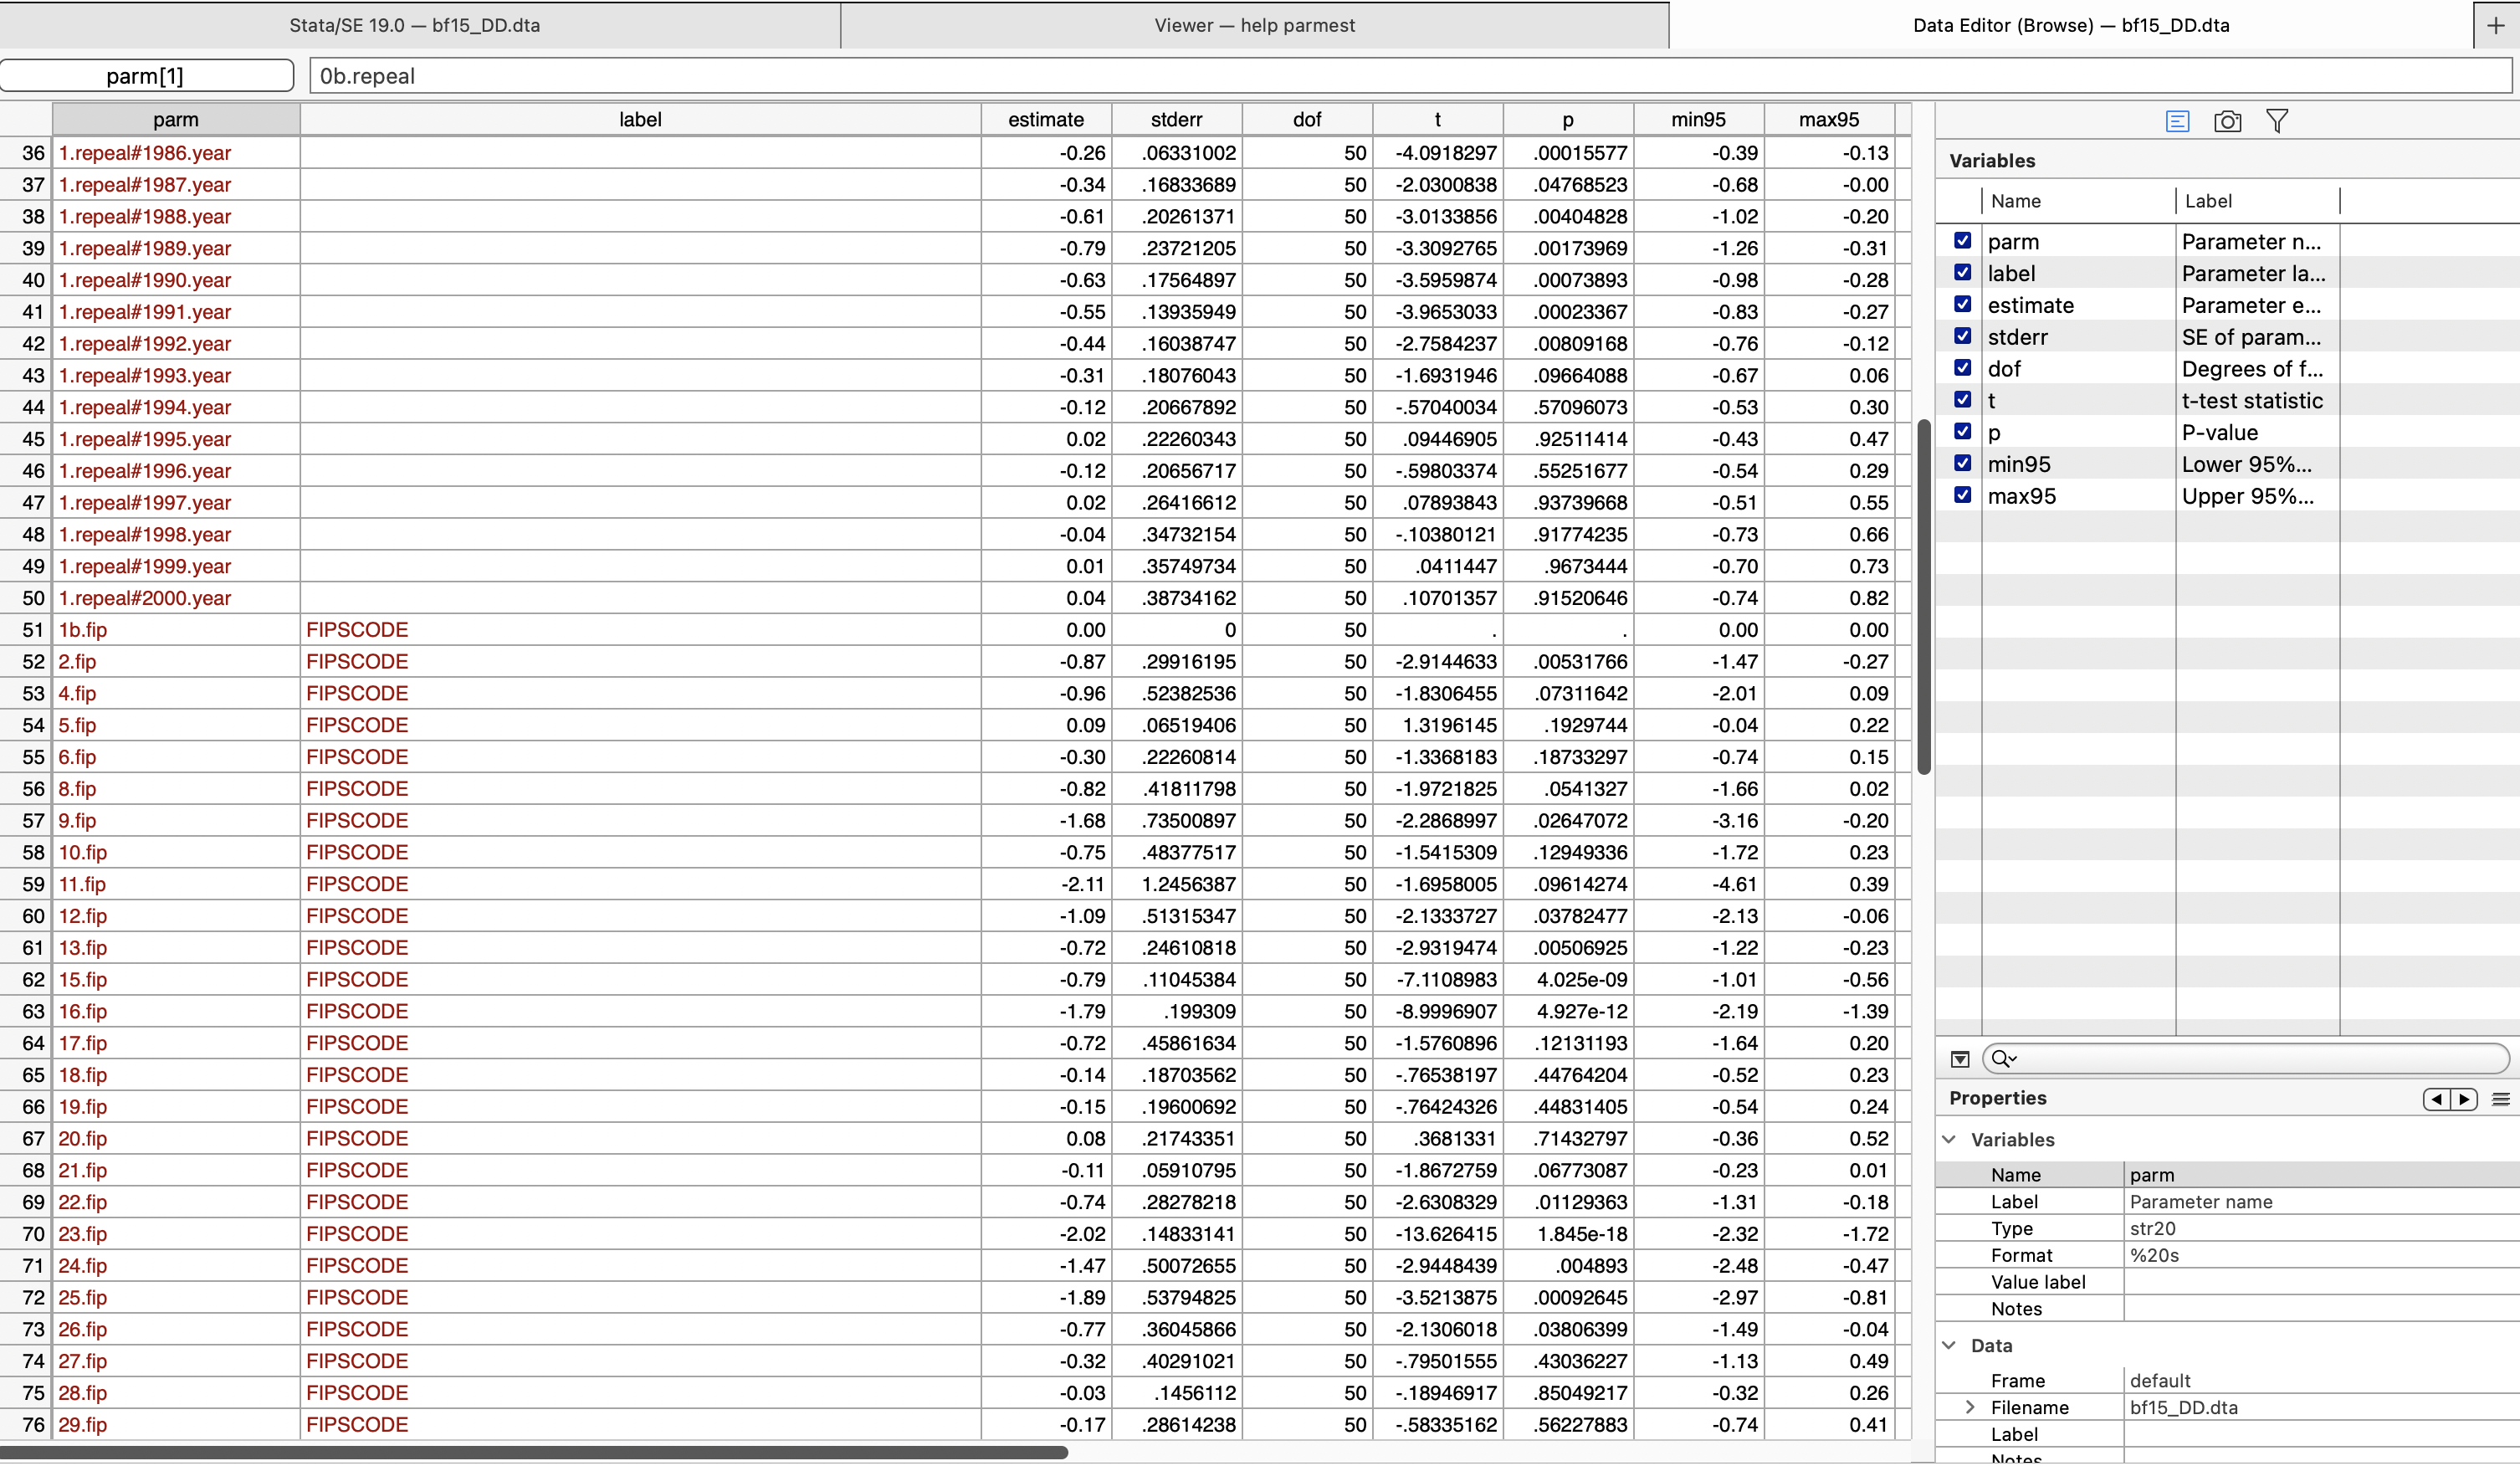
\includegraphics[keepaspectratio,alt={Parameter Estimates Output}]{DD2.png}}
\caption{Parameter Estimates Output}
\end{figure}

We will keep the difference-in-difference parameters, which are row 36 through row 50 observations.

\begin{Shaded}
\begin{Highlighting}[]
\KeywordTok{keep} \KeywordTok{in}\NormalTok{ 36/50}
\end{Highlighting}
\end{Shaded}

Next, we will generate a year variable for each year of the parameter estimates, and then we will sort the data.

\begin{Shaded}
\begin{Highlighting}[]
\NormalTok{*Generate }\FunctionTok{year} 
\KeywordTok{gen}     \FunctionTok{year}\NormalTok{=.}
\KeywordTok{replace} \FunctionTok{year}\NormalTok{=1986 }\KeywordTok{in}\NormalTok{ 1}
\KeywordTok{replace} \FunctionTok{year}\NormalTok{=1987 }\KeywordTok{in}\NormalTok{ 2}
\KeywordTok{replace} \FunctionTok{year}\NormalTok{=1988 }\KeywordTok{in}\NormalTok{ 3}
\KeywordTok{replace} \FunctionTok{year}\NormalTok{=1989 }\KeywordTok{in}\NormalTok{ 4}
\KeywordTok{replace} \FunctionTok{year}\NormalTok{=1990 }\KeywordTok{in}\NormalTok{ 5}
\KeywordTok{replace} \FunctionTok{year}\NormalTok{=1991 }\KeywordTok{in}\NormalTok{ 6}
\KeywordTok{replace} \FunctionTok{year}\NormalTok{=1992 }\KeywordTok{in}\NormalTok{ 7}
\KeywordTok{replace} \FunctionTok{year}\NormalTok{=1993 }\KeywordTok{in}\NormalTok{ 8}
\KeywordTok{replace} \FunctionTok{year}\NormalTok{=1994 }\KeywordTok{in}\NormalTok{ 9}
\KeywordTok{replace} \FunctionTok{year}\NormalTok{=1995 }\KeywordTok{in}\NormalTok{ 10}
\KeywordTok{replace} \FunctionTok{year}\NormalTok{=1996 }\KeywordTok{in}\NormalTok{ 11}
\KeywordTok{replace} \FunctionTok{year}\NormalTok{=1997 }\KeywordTok{in}\NormalTok{ 12}
\KeywordTok{replace} \FunctionTok{year}\NormalTok{=1998 }\KeywordTok{in}\NormalTok{ 13}
\KeywordTok{replace} \FunctionTok{year}\NormalTok{=1999 }\KeywordTok{in}\NormalTok{ 14}
\KeywordTok{replace} \FunctionTok{year}\NormalTok{=2000 }\KeywordTok{in}\NormalTok{ 15}

\KeywordTok{sort} \FunctionTok{year}
\end{Highlighting}
\end{Shaded}

Now we will graph our parameters using a twoway graph

\begin{Shaded}
\begin{Highlighting}[]
\KeywordTok{twoway}\NormalTok{ (}\KeywordTok{scatter}\NormalTok{ estimate }\FunctionTok{year}\NormalTok{, }\BaseNTok{mlabel}\NormalTok{(}\FunctionTok{year}\NormalTok{) }\BaseNTok{mlabsize}\NormalTok{(vsmall) msize(tiny)) }\CommentTok{///}
\NormalTok{  (rcap min95 max95 }\FunctionTok{year}\NormalTok{, msize(vsmall)), }\BaseNTok{ytitle}\NormalTok{(Repeal x }\FunctionTok{year}\NormalTok{ estimated coefficient) }\CommentTok{///}
  \BaseNTok{yscale}\NormalTok{(titlegap(2)) }\KeywordTok{yline}\NormalTok{(0, lwidth(thin) lcolor(}\BaseNTok{black}\NormalTok{)) }\BaseNTok{xtitle}\NormalTok{(Year) }\CommentTok{///}
  \BaseNTok{xline}\NormalTok{(1986 1987 1988 1989 1990 1991 1992, lwidth(vvvthick) }\CommentTok{///}
\NormalTok{  lpattern(solid) lcolor(}\BaseNTok{ltblue}\NormalTok{)) }\BaseNTok{xscale}\NormalTok{(titlegap(2)) }\CommentTok{///}
  \BaseNTok{title}\NormalTok{(Estimated effect }\KeywordTok{of}\NormalTok{ abortion legalization }\KeywordTok{on}\NormalTok{ gonorrhea) }\CommentTok{///}
  \BaseNTok{subtitle}\NormalTok{(Black females 15{-}19 }\FunctionTok{year}\NormalTok{{-}olds) }\CommentTok{///}
  \KeywordTok{note}\NormalTok{(W/o XI; Whisker plots are estimated coefficients }\KeywordTok{of}\NormalTok{ DD estimator from Column b }\KeywordTok{of}\NormalTok{ Table 2.) }\CommentTok{///}
  \BaseNTok{legend}\NormalTok{(}\KeywordTok{off}\NormalTok{)}
\end{Highlighting}
\end{Shaded}

\begin{figure}
\centering
\pandocbounded{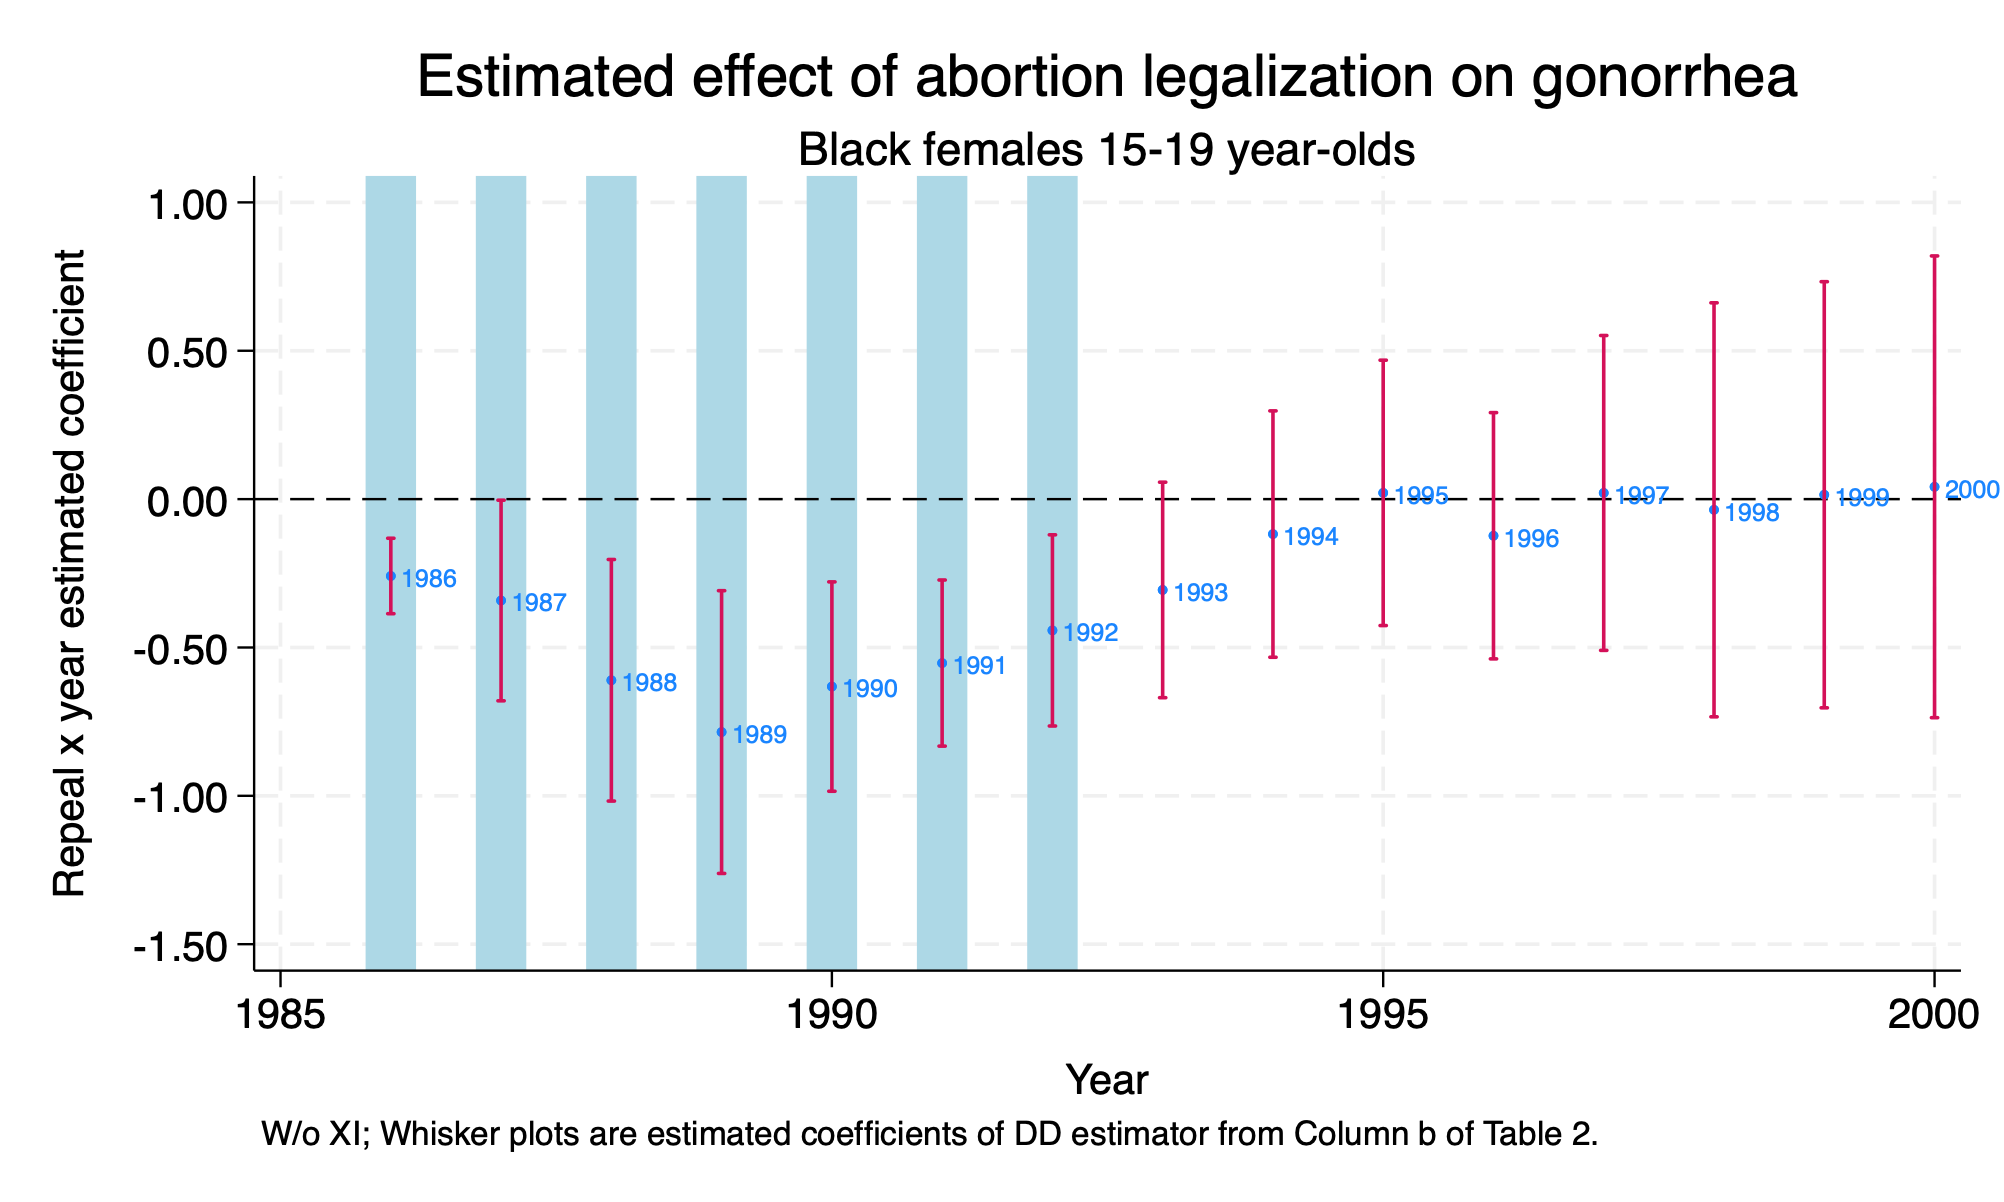
\includegraphics[keepaspectratio,alt={Difference-in-Differences Parameter Estimates 1986-2000}]{DD1.png}}
\caption{Difference-in-Differences Parameter Estimates 1986-2000}
\end{figure}

\chapter{Placebo Tests: False Treatment}\label{placebo-tests-false-treatment}

We have two major types of difference-in-differences placebo tests:

\begin{enumerate}
\def\labelenumi{\arabic{enumi}.}
\tightlist
\item
  False Treatment
\item
  False Timing
\end{enumerate}

\section{False Treatment}\label{false-treatment}

Our repeal states are Alaska (02), California (06), Hawaii (15), New York (36), Washington (53), so let's do false treatment placebo. We will assign Florida (12), Minnesota (27), Nevada (32), Ohio (39), and Pennsylvania (42) as our false treatment/repeal states.

\begin{Shaded}
\begin{Highlighting}[]
\KeywordTok{use} \StringTok{"/Users/Sam/Desktop/Econ 672/Data/abortion.dta"}\NormalTok{, }\KeywordTok{clear}

\KeywordTok{gen}\NormalTok{ repeal\_fake = 0}
\KeywordTok{replace}\NormalTok{ repeal\_fake = 1 }\KeywordTok{if}\NormalTok{ fip == 12}
\KeywordTok{replace}\NormalTok{ repeal\_fake = 1 }\KeywordTok{if}\NormalTok{ fip == 27}
\KeywordTok{replace}\NormalTok{ repeal\_fake = 1 }\KeywordTok{if}\NormalTok{ fip == 32}
\KeywordTok{replace}\NormalTok{ repeal\_fake = 1 }\KeywordTok{if}\NormalTok{ fip == 39}
\KeywordTok{replace}\NormalTok{ repeal\_fake = 1 }\KeywordTok{if}\NormalTok{ fip == 42}

\KeywordTok{tab}\NormalTok{ fip repeal\_fake}

\KeywordTok{reg}\NormalTok{ lnr i.repeal\_fake\#\#i.}\FunctionTok{year}\NormalTok{ i.fip acc }\KeywordTok{ir} \KeywordTok{pi}\NormalTok{ alcohol crack poverty income ur }\KeywordTok{if}\NormalTok{ bf15==1 [}\KeywordTok{aweight}\NormalTok{=totpop], }\KeywordTok{cluster}\NormalTok{(fip)}
\end{Highlighting}
\end{Shaded}

\begin{verbatim}
(384 real changes made)

(384 real changes made)

(384 real changes made)

(384 real changes made)

(384 real changes made)

           |      repeal_fake
  FIPSCODE |         0          1 |     Total
-----------+----------------------+----------
         1 |       384          0 |       384 
         2 |       384          0 |       384 
         4 |       384          0 |       384 
         5 |       384          0 |       384 
         6 |       384          0 |       384 
         8 |       384          0 |       384 
         9 |       384          0 |       384 
        10 |       384          0 |       384 
        11 |       384          0 |       384 
        12 |         0        384 |       384 
        13 |       384          0 |       384 
        15 |       384          0 |       384 
        16 |       384          0 |       384 
        17 |       384          0 |       384 
        18 |       384          0 |       384 
        19 |       384          0 |       384 
        20 |       384          0 |       384 
        21 |       384          0 |       384 
        22 |       384          0 |       384 
        23 |       384          0 |       384 
        24 |       384          0 |       384 
        25 |       384          0 |       384 
        26 |       384          0 |       384 
        27 |         0        384 |       384 
        28 |       384          0 |       384 
        29 |       384          0 |       384 
        30 |       384          0 |       384 
        31 |       384          0 |       384 
        32 |         0        384 |       384 
        33 |       384          0 |       384 
        34 |       384          0 |       384 
        35 |       384          0 |       384 
        36 |       384          0 |       384 
        37 |       384          0 |       384 
        38 |       384          0 |       384 
        39 |         0        384 |       384 
        40 |       384          0 |       384 
        41 |       384          0 |       384 
        42 |         0        384 |       384 
        44 |       384          0 |       384 
        45 |       384          0 |       384 
        46 |       384          0 |       384 
        47 |       384          0 |       384 
        48 |       384          0 |       384 
        49 |       384          0 |       384 
        50 |       384          0 |       384 
        51 |       384          0 |       384 
        53 |       384          0 |       384 
        54 |       384          0 |       384 
        55 |       384          0 |       384 
        56 |       384          0 |       384 
-----------+----------------------+----------
     Total |    17,664      1,920 |    19,584 

(sum of wgt is 43,100,087)
note: 42.fip omitted because of collinearity.

Linear regression                               Number of obs     =        736
                                                F(26, 50)         =          .
                                                Prob > F          =          .
                                                R-squared         =     0.8430
                                                Root MSE          =     .25494

                                    (Std. err. adjusted for 51 clusters in fip)
-------------------------------------------------------------------------------
              |               Robust
          lnr | Coefficient  std. err.      t    P>|t|     [95% conf. interval]
--------------+----------------------------------------------------------------
1.repeal_fake |  -.2619235   .3063582    -0.85   0.397     -.877262     .353415
              |
         year |
        1986  |  -.0473925   .0623881    -0.76   0.451    -.1727026    .0779176
        1987  |   -.282811   .1071218    -2.64   0.011    -.4979714   -.0676506
        1988  |  -.3047447   .1380771    -2.21   0.032    -.5820807   -.0274087
        1989  |  -.3381935   .1805399    -1.87   0.067    -.7008186    .0244316
        1990  |  -.3411266   .2247542    -1.52   0.135    -.7925586    .1103054
        1991  |  -.3638668   .2180394    -1.67   0.101    -.8018117    .0740781
        1992  |  -.5641131   .2553435    -2.21   0.032    -1.076986   -.0512405
        1993  |  -.6982166     .25845    -2.70   0.009    -1.217329   -.1791045
        1994  |   -.704213   .2728245    -2.58   0.013    -1.252197   -.1562289
        1995  |   -.938756   .3081557    -3.05   0.004    -1.557705   -.3198071
        1996  |  -1.085633   .3629182    -2.99   0.004    -1.814576   -.3566907
        1997  |  -1.069773   .4168856    -2.57   0.013    -1.907112   -.2324331
        1998  |  -1.006071   .4858285    -2.07   0.044    -1.981887   -.0302559
        1999  |  -1.017142   .5311595    -1.91   0.061    -2.084007     .049723
        2000  |  -1.062719   .5999853    -1.77   0.083    -2.267825    .1423874
              |
  repeal_fake#|
         year |
      1 1986  |   .1961008   .1580668     1.24   0.221    -.1213857    .5135873
      1 1987  |   .3019751   .1659506     1.82   0.075    -.0313465    .6352967
      1 1988  |   .1925532   .1376346     1.40   0.168     -.083894    .4690004
      1 1989  |   .2587087    .163867     1.58   0.121     -.070428    .5878453
      1 1990  |   .1725233   .1545046     1.12   0.269    -.1378082    .4828549
      1 1991  |   .0588022   .1357068     0.43   0.667    -.2137729    .3313773
      1 1992  |  -.0298446    .148425    -0.20   0.841    -.3279649    .2682758
      1 1993  |  -.0782904   .1372765    -0.57   0.571    -.3540183    .1974375
      1 1994  |  -.0599632    .123157    -0.49   0.628    -.3073313    .1874049
      1 1995  |   .0068644    .145227     0.05   0.962    -.2848327    .2985614
      1 1996  |    .006097   .1133758     0.05   0.957     -.221625     .233819
      1 1997  |  -.0625821   .1155086    -0.54   0.590     -.294588    .1694237
      1 1998  |  -.0846898   .1382085    -0.61   0.543    -.3622897    .1929101
      1 1999  |  -.0037381   .1298435    -0.03   0.977    -.2645364    .2570603
      1 2000  |   .0295735   .1186556     0.25   0.804    -.2087532    .2679002
              |
          fip |
           2  |   -1.67931   .7013951    -2.39   0.020    -3.088104   -.2705167
           4  |  -.4782904   .4415301    -1.08   0.284     -1.36513    .4085488
           5  |   .0570652   .0799359     0.71   0.479    -.1034908    .2176211
           6  |  -.9959097   .5272526    -1.89   0.065    -2.054928    .0631083
           8  |  -.5320145   .4589932    -1.16   0.252     -1.45393    .3899005
           9  |  -.9013381   .7003092    -1.29   0.204    -2.307951    .5052743
          10  |  -.3408189   .5989758    -0.57   0.572    -1.543897    .8622595
          11  |  -1.319298   1.324266    -1.00   0.324    -3.979165    1.340569
          12  |  -.4700227   .2584934    -1.82   0.075     -.989222    .0491766
          13  |  -.4658355   .2632261    -1.77   0.083    -.9945406    .0628696
          15  |  -1.712506   .4372031    -3.92   0.000    -2.590654   -.8343573
          16  |  -1.698102   .1825109    -9.30   0.000    -2.064686   -1.331518
          17  |  -.3702913   .4493088    -0.82   0.414    -1.272755     .532172
          18  |   .1378953   .1998675     0.69   0.493    -.2635504    .5393411
          19  |   .0936967   .1653353     0.57   0.573     -.238389    .4257823
          20  |   .3886963   .1730131     2.25   0.029     .0411892    .7362035
          21  |  -.0840023    .056987    -1.47   0.147    -.1984641    .0304594
          22  |   -.623181   .2715091    -2.30   0.026    -1.168523   -.0778389
          23  |  -2.043909   .2082448    -9.81   0.000    -2.462181   -1.625637
          24  |  -.9304013   .5056388    -1.84   0.072    -1.946007    .0852041
          25  |  -1.362687   .6297522    -2.16   0.035    -2.627582   -.0977927
          26  |  -.4230176   .3390352    -1.25   0.218     -1.10399    .2579546
          27  |   .2942861   .1721111     1.71   0.093    -.0514092    .6399814
          28  |  -.1631074    .132844    -1.23   0.225    -.4299325    .1037176
          29  |   .1893571   .2860834     0.66   0.511    -.3852584    .7639725
          30  |  -1.350451    .248263    -5.44   0.000    -1.849102   -.8518006
          31  |   .2705925   .2813189     0.96   0.341     -.294453    .8356381
          32  |  -1.022858   .8797807    -1.16   0.250    -2.789949     .744234
          33  |  -3.093851   1.071677    -2.89   0.006    -5.246377   -.9413251
          34  |  -1.651775   .6231486    -2.65   0.011    -2.903406   -.4001445
          35  |  -1.024749   .2929583    -3.50   0.001    -1.613173   -.4363253
          36  |  -2.118819   .4655078    -4.55   0.000    -3.053819    -1.18382
          37  |   .0543435   .1264402     0.43   0.669    -.1996191     .308306
          38  |   -1.83464   .2001633    -9.17   0.000     -2.23668     -1.4326
          39  |   .0414655   .0717687     0.58   0.566    -.1026862    .1856172
          40  |   .3004358   .0858056     3.50   0.001     .1280901    .4727815
          41  |  -.7933867   .3571316    -2.22   0.031    -1.510707   -.0760667
          42  |          0  (omitted)
          44  |  -.5405153   .5104011    -1.06   0.295    -1.565686    .4846555
          45  |  -.9602952   .2294899    -4.18   0.000    -1.421239   -.4993512
          46  |  -1.127867   .4597007    -2.45   0.018    -2.051204   -.2045314
          47  |   .1312519   .0886643     1.48   0.145    -.0468356    .3093394
          48  |  -.3837915   .3086508    -1.24   0.220    -1.003735    .2361518
          49  |   -.966726   .2534117    -3.81   0.000    -1.475718   -.4577335
          50  |  -1.942943   .3250246    -5.98   0.000    -2.595774   -1.290112
          51  |  -.5903806   .3069945    -1.92   0.060    -1.206997     .026236
          53  |  -.8368507   .4010224    -2.09   0.042    -1.642328   -.0313735
          54  |  -.5250537   .1220392    -4.30   0.000    -.7701766   -.2799308
          55  |   .1296001   .5587953     0.23   0.818    -.9927732    1.251973
          56  |  -1.497547   .4613406    -3.25   0.002    -2.424176   -.5709167
              |
          acc |   .0017173   .0010087     1.70   0.095    -.0003087    .0037433
           ir |  -.0001316   .0002427    -0.54   0.590    -.0006192     .000356
           pi |  -.1012491   .0940607    -1.08   0.287    -.2901756    .0876774
      alcohol |   .3243983   .3896246     0.83   0.409    -.4581858    1.106982
        crack |   .0406948   .0415672     0.98   0.332    -.0427954     .124185
      poverty |   .0089868   .0164328     0.55   0.587    -.0240195    .0419931
       income |   .0000331   .0000418     0.79   0.432    -.0000508    .0001171
           ur |  -.0143629   .0374348    -0.38   0.703    -.0895528    .0608271
        _cons |   7.790753   1.229231     6.34   0.000      5.32177    10.25974
-------------------------------------------------------------------------------
\end{verbatim}

Again, we will save the parameter estimates, keep the difference-in-difference parameters, and graph our results.

\begin{Shaded}
\begin{Highlighting}[]
\NormalTok{parmest, }\KeywordTok{label} \KeywordTok{for}\NormalTok{(estimate min95 max95 \%8.2f) li(parm }\KeywordTok{label}\NormalTok{ estimate min95 max95) }\CommentTok{///}
 \KeywordTok{saving}\NormalTok{(bf15\_DD\_false.dta, }\KeywordTok{replace}\NormalTok{)}
 
\KeywordTok{use}\NormalTok{ ./bf15\_DD\_false.dta, }\KeywordTok{replace}  
\end{Highlighting}
\end{Shaded}

Keep the Diff-in-Diff Interaction Parameter Estimates and generate a year variable

\begin{Shaded}
\begin{Highlighting}[]
\KeywordTok{keep} \KeywordTok{in}\NormalTok{ 36/50}

\KeywordTok{gen}     \FunctionTok{year}\NormalTok{=.}
\KeywordTok{replace} \FunctionTok{year}\NormalTok{=1986 }\KeywordTok{in}\NormalTok{ 1}
\KeywordTok{replace} \FunctionTok{year}\NormalTok{=1987 }\KeywordTok{in}\NormalTok{ 2}
\KeywordTok{replace} \FunctionTok{year}\NormalTok{=1988 }\KeywordTok{in}\NormalTok{ 3}
\KeywordTok{replace} \FunctionTok{year}\NormalTok{=1989 }\KeywordTok{in}\NormalTok{ 4}
\KeywordTok{replace} \FunctionTok{year}\NormalTok{=1990 }\KeywordTok{in}\NormalTok{ 5}
\KeywordTok{replace} \FunctionTok{year}\NormalTok{=1991 }\KeywordTok{in}\NormalTok{ 6}
\KeywordTok{replace} \FunctionTok{year}\NormalTok{=1992 }\KeywordTok{in}\NormalTok{ 7}
\KeywordTok{replace} \FunctionTok{year}\NormalTok{=1993 }\KeywordTok{in}\NormalTok{ 8}
\KeywordTok{replace} \FunctionTok{year}\NormalTok{=1994 }\KeywordTok{in}\NormalTok{ 9}
\KeywordTok{replace} \FunctionTok{year}\NormalTok{=1995 }\KeywordTok{in}\NormalTok{ 10}
\KeywordTok{replace} \FunctionTok{year}\NormalTok{=1996 }\KeywordTok{in}\NormalTok{ 11}
\KeywordTok{replace} \FunctionTok{year}\NormalTok{=1997 }\KeywordTok{in}\NormalTok{ 12}
\KeywordTok{replace} \FunctionTok{year}\NormalTok{=1998 }\KeywordTok{in}\NormalTok{ 13}
\KeywordTok{replace} \FunctionTok{year}\NormalTok{=1999 }\KeywordTok{in}\NormalTok{ 14}
\KeywordTok{replace} \FunctionTok{year}\NormalTok{=2000 }\KeywordTok{in}\NormalTok{ 15}
\end{Highlighting}
\end{Shaded}

Finally, we will sort and graph our data.

\begin{Shaded}
\begin{Highlighting}[]
\KeywordTok{sort} \FunctionTok{year}

\NormalTok{*Graph Parameter Estimates with Confidence Intervals}
\KeywordTok{twoway}\NormalTok{ (}\KeywordTok{scatter}\NormalTok{ estimate }\FunctionTok{year}\NormalTok{, }\BaseNTok{mlabel}\NormalTok{(}\FunctionTok{year}\NormalTok{) }\BaseNTok{mlabsize}\NormalTok{(vsmall) msize(tiny)) }\CommentTok{///}
\NormalTok{  (rcap min95 max95 }\FunctionTok{year}\NormalTok{, msize(vsmall)), }\BaseNTok{ytitle}\NormalTok{(Repeal x }\FunctionTok{year}\NormalTok{ estimated coefficient) }\CommentTok{///}
  \BaseNTok{yscale}\NormalTok{(titlegap(2)) }\KeywordTok{yline}\NormalTok{(0, lwidth(thin) lcolor(}\BaseNTok{black}\NormalTok{)) }\BaseNTok{xtitle}\NormalTok{(Year) }\CommentTok{///}
  \BaseNTok{xline}\NormalTok{(1986 1987 1988 1989 1990 1991 1992, lwidth(vvvthick) }\CommentTok{///}
\NormalTok{  lpattern(solid) lcolor(}\BaseNTok{ltblue}\NormalTok{)) }\BaseNTok{xscale}\NormalTok{(titlegap(2)) }\CommentTok{///}
  \BaseNTok{title}\NormalTok{(Placebo Test: Fake Treatment }\KeywordTok{of}\NormalTok{ abortion legalization }\KeywordTok{on}\NormalTok{ gonorrhea) }\CommentTok{///}
  \BaseNTok{subtitle}\NormalTok{(Black females 15{-}19 }\FunctionTok{year}\NormalTok{{-}olds) }\CommentTok{///}
  \KeywordTok{note}\NormalTok{(W/o XI; Wh}
\end{Highlighting}
\end{Shaded}

\begin{figure}
\centering
\pandocbounded{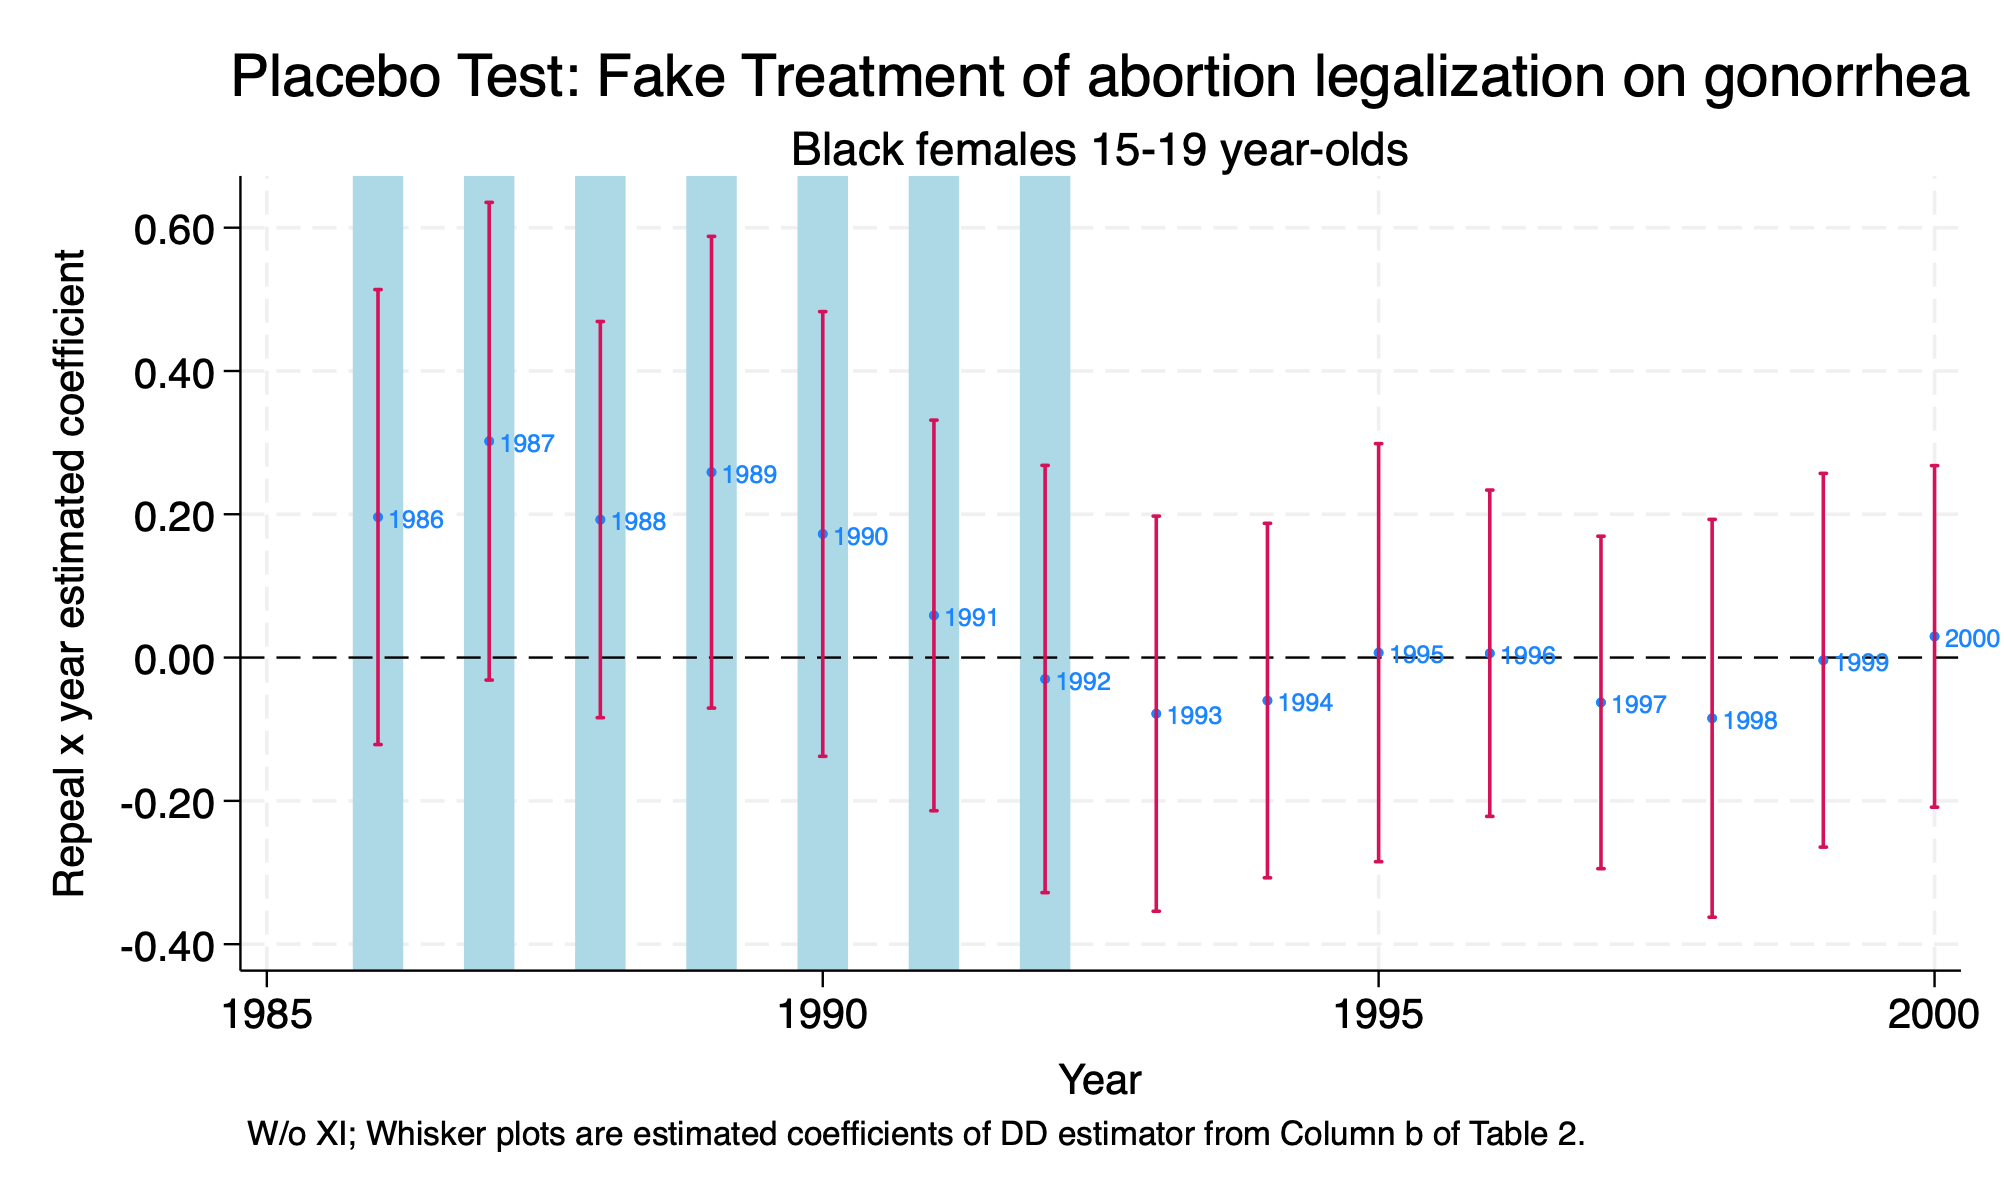
\includegraphics[keepaspectratio,alt={Placebo Test: False Treatment}]{DD3.png}}
\caption{Placebo Test: False Treatment}
\end{figure}

In support of Cunningham and Cormwell's hypothesis, we fail to reject the null hypothesis at the 5 percent level across the years.

\chapter{\texorpdfstring{\emph{xtdidregress} commmands}{xtdidregress commmands}}\label{xtdidregress-commmands}

In addition to using \emph{xtreg} or \emph{reg} for estimating our \(\delta^{ATET}_{DD}\), we can use some built in Stata commands instead. These commands include \emph{xtdidregress} and \emph{didregress}.

For additional information we can use the \emph{help} command.

\begin{Shaded}
\begin{Highlighting}[]
\KeywordTok{help}\NormalTok{ didregress}
\end{Highlighting}
\end{Shaded}

Stata's help page provides us with the following information:

For repeated cross-sections:

\textbf{didregress} (\emph{ovar omvarlist}) (\emph{tvar}{[}, \textbf{continuous}{]}) {[}\emph{if}{]} {[}\emph{in}{]} {[}\emph{weight}{]}, \textbf{group}(\emph{groupvars}) {[}\textbf{time}(\emph{timevar}) \emph{options}{]}

For panel data:

\textbf{xtdidregress} (\emph{ovar omvarlist}) (\emph{tvar}{[}, \textbf{continuous}{]}) {[}\emph{if}{]} {[}\emph{in}{]} {[}\emph{weight}{]}, \textbf{group}(\emph{groupvars}) {[}\textbf{time}(\emph{timevar}) \emph{options}{]}

Where
1. \emph{ovar} is our outcome of interest
2. \emph{omvarlist} is a list of our explanatory covariates
3. \emph{tvar} is a binary indicating treatment status or a continuous indicating intensity of treatment
4. \emph{groupvars} are categorical variables indicating treatment level, such as individual, state, etc.
5. \emph{timevar} is our time variable, such as year

\section{World Development Index}\label{world-development-index}

We will use the World Development Index to assess the impact of a trade policy in 2000 on total amount of trade (imports + exports) in millions of 2005 US dollars. These data are provided by Princeton.

\begin{Shaded}
\begin{Highlighting}[]
\NormalTok{cd }\StringTok{"/Users/Sam/Desktop/Econ 672/Data/"}
\KeywordTok{use}\NormalTok{ wdipol, }\KeywordTok{clear}
\KeywordTok{describe}
\end{Highlighting}
\end{Shaded}

\begin{verbatim}
/Users/Sam/Desktop/Econ 672/Data



Contains data from wdipol.dta
 Observations:         4,542                  
    Variables:            12                  26 Mar 2026 19:15
----------------------------------------------------------------------------------
Variable      Storage   Display    Value
    name         type    format    label      Variable label
----------------------------------------------------------------------------------
year            int     %10.0g                Year
country         str24   %24s                  Country Name
gdppc           double  %10.0g                 GDP per capita, PPP (constant 2005
                                                international $)
unempf          double  %10.0g                Unemployment, female (% of female
                                                labor force)
unempm          double  %10.0g                Unemployment, male (% of male labor
                                                force)
unemp           double  %10.0g                Unemployment, total (% of total
                                                labor force)
export          double  %10.0g                Exports of goods and services
                                                (constant 2005 US$)
import          double  %10.0g                Imports of goods and services
                                                (constant 2005 US$)
polity          byte    %8.0g                 polity (original)
polity2         byte    %8.0g                 polity2 (adjusted)
trade           float   %9.0g                 Imports + Exports
id              float   %9.0g                 group(country)
----------------------------------------------------------------------------------
Sorted by: 
\end{verbatim}

We will focus on years 1990 forward.

\begin{Shaded}
\begin{Highlighting}[]
\KeywordTok{drop} \KeywordTok{if} \FunctionTok{year}\NormalTok{ \textless{} 1990}
\KeywordTok{sum} \KeywordTok{export}\NormalTok{ import trade, }\KeywordTok{detail}
\end{Highlighting}
\end{Shaded}

\begin{verbatim}
(1,136 observations deleted)

      Exports of goods and services (constant 2005 US$)
-------------------------------------------------------------
      Percentiles      Smallest
 1%     91.64278       45.02022
 5%     245.0359       48.62297
10%     543.8475       52.79048       Obs               2,814
25%     2094.341       53.24336       Sum of wgt.       2,814

50%     8836.828                      Mean           75432.49
                        Largest       Std. dev.      182677.6
75%     57261.36        1649300
90%     198699.2        1665600       Variance       3.34e+10
95%     399759.2        1677840       Skewness       4.764539
99%      1036798        1776900       Kurtosis       31.56892

      Imports of goods and services (constant 2005 US$)
-------------------------------------------------------------
      Percentiles      Smallest
 1%     264.6554       94.23958
 5%     538.7271       110.3702
10%     1031.108       129.2793       Obs               2,814
25%     2514.115       135.4336       Sum of wgt.       2,814

50%      10218.4                      Mean           74643.16
                        Largest       Std. dev.        194233
75%     56131.35        2144000
90%     182048.5        2151500       Variance       3.77e+10
95%     371224.2        2184900       Skewness       5.811369
99%       943900        2203200       Kurtosis       47.77702

                      Imports + Exports
-------------------------------------------------------------
      Percentiles      Smallest
 1%     414.4894       139.2598
 5%     828.4978       166.8271
10%      1613.88       183.3966       Obs               2,814
25%     4867.792       193.1237       Sum of wgt.       2,814

50%     19421.02                      Mean           150075.7
                        Largest       Std. dev.      374324.7
75%     115498.2        3750800
90%     382896.8        3757600       Variance       1.40e+11
95%     759593.4        3793300       Skewness       5.158498
99%      2001955        3961800       Kurtosis       37.13028
\end{verbatim}

Looking at combined imports and exports, the median amount of trade is 19.4 billion 2005 US dollars.

Now, we set our post period at 2000 or later. An indicator for when trade relations were normalized between the U.S. and China and China's ascension into the World Trade Organization (WTO).

\begin{Shaded}
\begin{Highlighting}[]
\KeywordTok{gen} \KeywordTok{post}\NormalTok{ = .}
\KeywordTok{replace} \KeywordTok{post}\NormalTok{ = 0 }\KeywordTok{if} \FunctionTok{year}\NormalTok{ \textless{} 2000}
\KeywordTok{replace} \KeywordTok{post}\NormalTok{ = 1 }\KeywordTok{if} \FunctionTok{year}\NormalTok{ \textgreater{}= 2000}
\end{Highlighting}
\end{Shaded}

Next we will assign the treatment countries, which are the following western countries: Australia, Austria, Belgium, Canada, Denmark, Finland, France, Germany, Greece, Ireland, Italy, Luxembourg, Netherlands, New Zealand, Norway, Portugal, Spain, Sweden, Switzerland, United Kingdom, and United States.

\begin{Shaded}
\begin{Highlighting}[]
\KeywordTok{gen}\NormalTok{ treatment = 0}
\KeywordTok{replace}\NormalTok{ treatment = 1 }\KeywordTok{if}\NormalTok{ country == }\StringTok{"Australia"}\NormalTok{ | country == }\StringTok{"Austria"}\NormalTok{ | country == }\StringTok{"Belgium"}\NormalTok{ | country == }\StringTok{"Canada"}\NormalTok{ | country == }\StringTok{"Denmark"}\NormalTok{ | country == }\StringTok{"Finland"}\NormalTok{ | country == }\StringTok{"France"}\NormalTok{ | country == }\StringTok{"Germany"}\NormalTok{ | country == }\StringTok{"Greece"}\NormalTok{ | country == }\StringTok{"Ireland"}\NormalTok{ | country == }\StringTok{"Italy"}\NormalTok{ | country == }\StringTok{"Luxembourg"}\NormalTok{ | country == }\StringTok{"Netherlands"}\NormalTok{ | country == }\StringTok{"New Zealand"}\NormalTok{ | country == }\StringTok{"Norway"}\NormalTok{ | country == }\StringTok{"Portugal"}\NormalTok{ | country == }\StringTok{"Spain"}\NormalTok{ |country == }\StringTok{"Sweden"}\NormalTok{ | country == }\StringTok{"Switzerland"}\NormalTok{ | country == }\StringTok{"United Kingdom"}\NormalTok{ | country == }\StringTok{"United States"}
\end{Highlighting}
\end{Shaded}

Next, we will set up the difference-in-differences interaction.

\begin{Shaded}
\begin{Highlighting}[]
\KeywordTok{gen}\NormalTok{ treat\_post=treatment*}\KeywordTok{post}
\end{Highlighting}
\end{Shaded}

Now we need to establish our panel, but we need to use the \emph{encode} command on countries so we can use the \emph{xtset} command.

\begin{Shaded}
\begin{Highlighting}[]
\NormalTok{*Encode country}
\KeywordTok{encode}\NormalTok{ country, }\KeywordTok{gen}\NormalTok{(countrynum)}

\NormalTok{*Set Panel}
\KeywordTok{sort}\NormalTok{ countrynum }\FunctionTok{year}
\NormalTok{xtset countrynum }\FunctionTok{year}
\end{Highlighting}
\end{Shaded}

\begin{verbatim}
Panel variable: countrynum (unbalanced)
 Time variable: year, 1990 to 2012, but with a gap
         Delta: 1 unit
\end{verbatim}

Our panel is unbalanced, which means we do have gaps among some of the countries.

We will first start with our tried and true method with \emph{xtreg} and use the \emph{fe} option, and we will cluster our standard errors at the unit of observation level.

\begin{Shaded}
\begin{Highlighting}[]
\KeywordTok{xtreg}\NormalTok{ trade treat\_post i.}\FunctionTok{year}\NormalTok{, }\KeywordTok{fe} \KeywordTok{vce}\NormalTok{ (}\KeywordTok{cluster}\NormalTok{ countrynum)}
\end{Highlighting}
\end{Shaded}

\begin{verbatim}
Fixed-effects (within) regression               Number of obs     =      2,814
Group variable: countrynum                      Number of groups  =        153

R-squared:                                      Obs per group:
     Within  = 0.2476                                         min =          1
     Between = 0.2331                                         avg =       18.4
     Overall = 0.1877                                         max =         23

                                                F(23, 152)        =       2.88
corr(u_i, Xb) = 0.2187                          Prob > F          =     0.0001

                           (Std. err. adjusted for 153 clusters in countrynum)
------------------------------------------------------------------------------
             |               Robust
       trade | Coefficient  std. err.      t    P>|t|     [95% conf. interval]
-------------+----------------------------------------------------------------
  treat_post |   254619.5   84665.83     3.01   0.003     87345.69    421893.2
             |
        year |
       1991  |   11417.79   3273.274     3.49   0.001     4950.798    17884.77
       1992  |   14691.17   4183.539     3.51   0.001     6425.782    22956.57
       1993  |   17823.51   5089.347     3.50   0.001     7768.513     27878.5
       1994  |   27212.01   6768.259     4.02   0.000     13840.01    40584.02
       1995  |   36908.65   8577.682     4.30   0.000     19961.77    53855.52
       1996  |    43697.3   9997.622     4.37   0.000     23945.06    63449.54
       1997  |   53882.39   12313.33     4.38   0.000     29555.02    78209.75
       1998  |   60352.96   13818.67     4.37   0.000      33051.5    87654.42
       1999  |   67276.08   15777.22     4.26   0.000     36105.13    98447.04
       2000  |   43940.78   12961.89     3.39   0.001     18332.06     69549.5
       2001  |   45574.41   13023.31     3.50   0.001     19844.34    71304.49
       2002  |   50357.95    14195.9     3.55   0.001     22311.21     78404.7
       2003  |   58200.38    16052.8     3.63   0.000     26484.97    89915.79
       2004  |   74493.25   18905.12     3.94   0.000     37142.52      111844
       2005  |    87670.9   21325.73     4.11   0.000     45537.78      129804
       2006  |   104994.9   24623.44     4.26   0.000     56346.51    153643.3
       2007  |   121106.3   28005.54     4.32   0.000     65775.88    176436.6
       2008  |   128370.5   29721.71     4.32   0.000     69649.48    187091.5
       2009  |   104644.4   27073.14     3.87   0.000     51156.19    158132.7
       2010  |   131099.8   33071.58     3.96   0.000     65760.48    196439.1
       2011  |   149272.6   37479.36     3.98   0.000     75224.91    223320.4
       2012  |   129456.8   24816.73     5.22   0.000     80426.54    178487.1
             |
       _cons |   56946.96   18846.82     3.02   0.003     19711.41    94182.51
-------------+----------------------------------------------------------------
     sigma_u |  295226.32
     sigma_e |   132684.6
         rho |  .83195335   (fraction of variance due to u_i)
------------------------------------------------------------------------------
\end{verbatim}

Our difference-in-difference estimator indicates that the change in trade policy increased total trade by 255 billion 2005 US dollars, which is statistically significant at the 1\% level.

To visualize our parallel trends, we need to use \emph{egen} to get the mean outcome by year for treatment and comparison groups. Next, we will visually inspect the parallel trends assumption with \emph{twoway line} charts.

\begin{Shaded}
\begin{Highlighting}[]
\KeywordTok{bysort} \FunctionTok{year}\NormalTok{ treatment: }\KeywordTok{egen}\NormalTok{ mean\_trade = }\KeywordTok{mean}\NormalTok{(trade)}

\KeywordTok{twoway} \KeywordTok{line}\NormalTok{ mean\_trade }\FunctionTok{year} \KeywordTok{if}\NormalTok{ treatment == 0, }\KeywordTok{sort}\NormalTok{ || }\CommentTok{///}
       \KeywordTok{line}\NormalTok{ mean\_trade }\FunctionTok{year} \KeywordTok{if}\NormalTok{ treatment == 1, }\KeywordTok{sort}\NormalTok{ lpattern (}\KeywordTok{dash}\NormalTok{) }\CommentTok{///}
       \BaseNTok{legend}\NormalTok{(}\KeywordTok{label}\NormalTok{(1 }\StringTok{"Control"}\NormalTok{) }\KeywordTok{label}\NormalTok{(2 }\StringTok{"Treated"}\NormalTok{)) }\CommentTok{///}
       \BaseNTok{xline}\NormalTok{(2000) }\BaseNTok{title}\NormalTok{(}\StringTok{"Check Parallel Trends Assumption"}\NormalTok{)}
\end{Highlighting}
\end{Shaded}

\begin{figure}
\centering
\pandocbounded{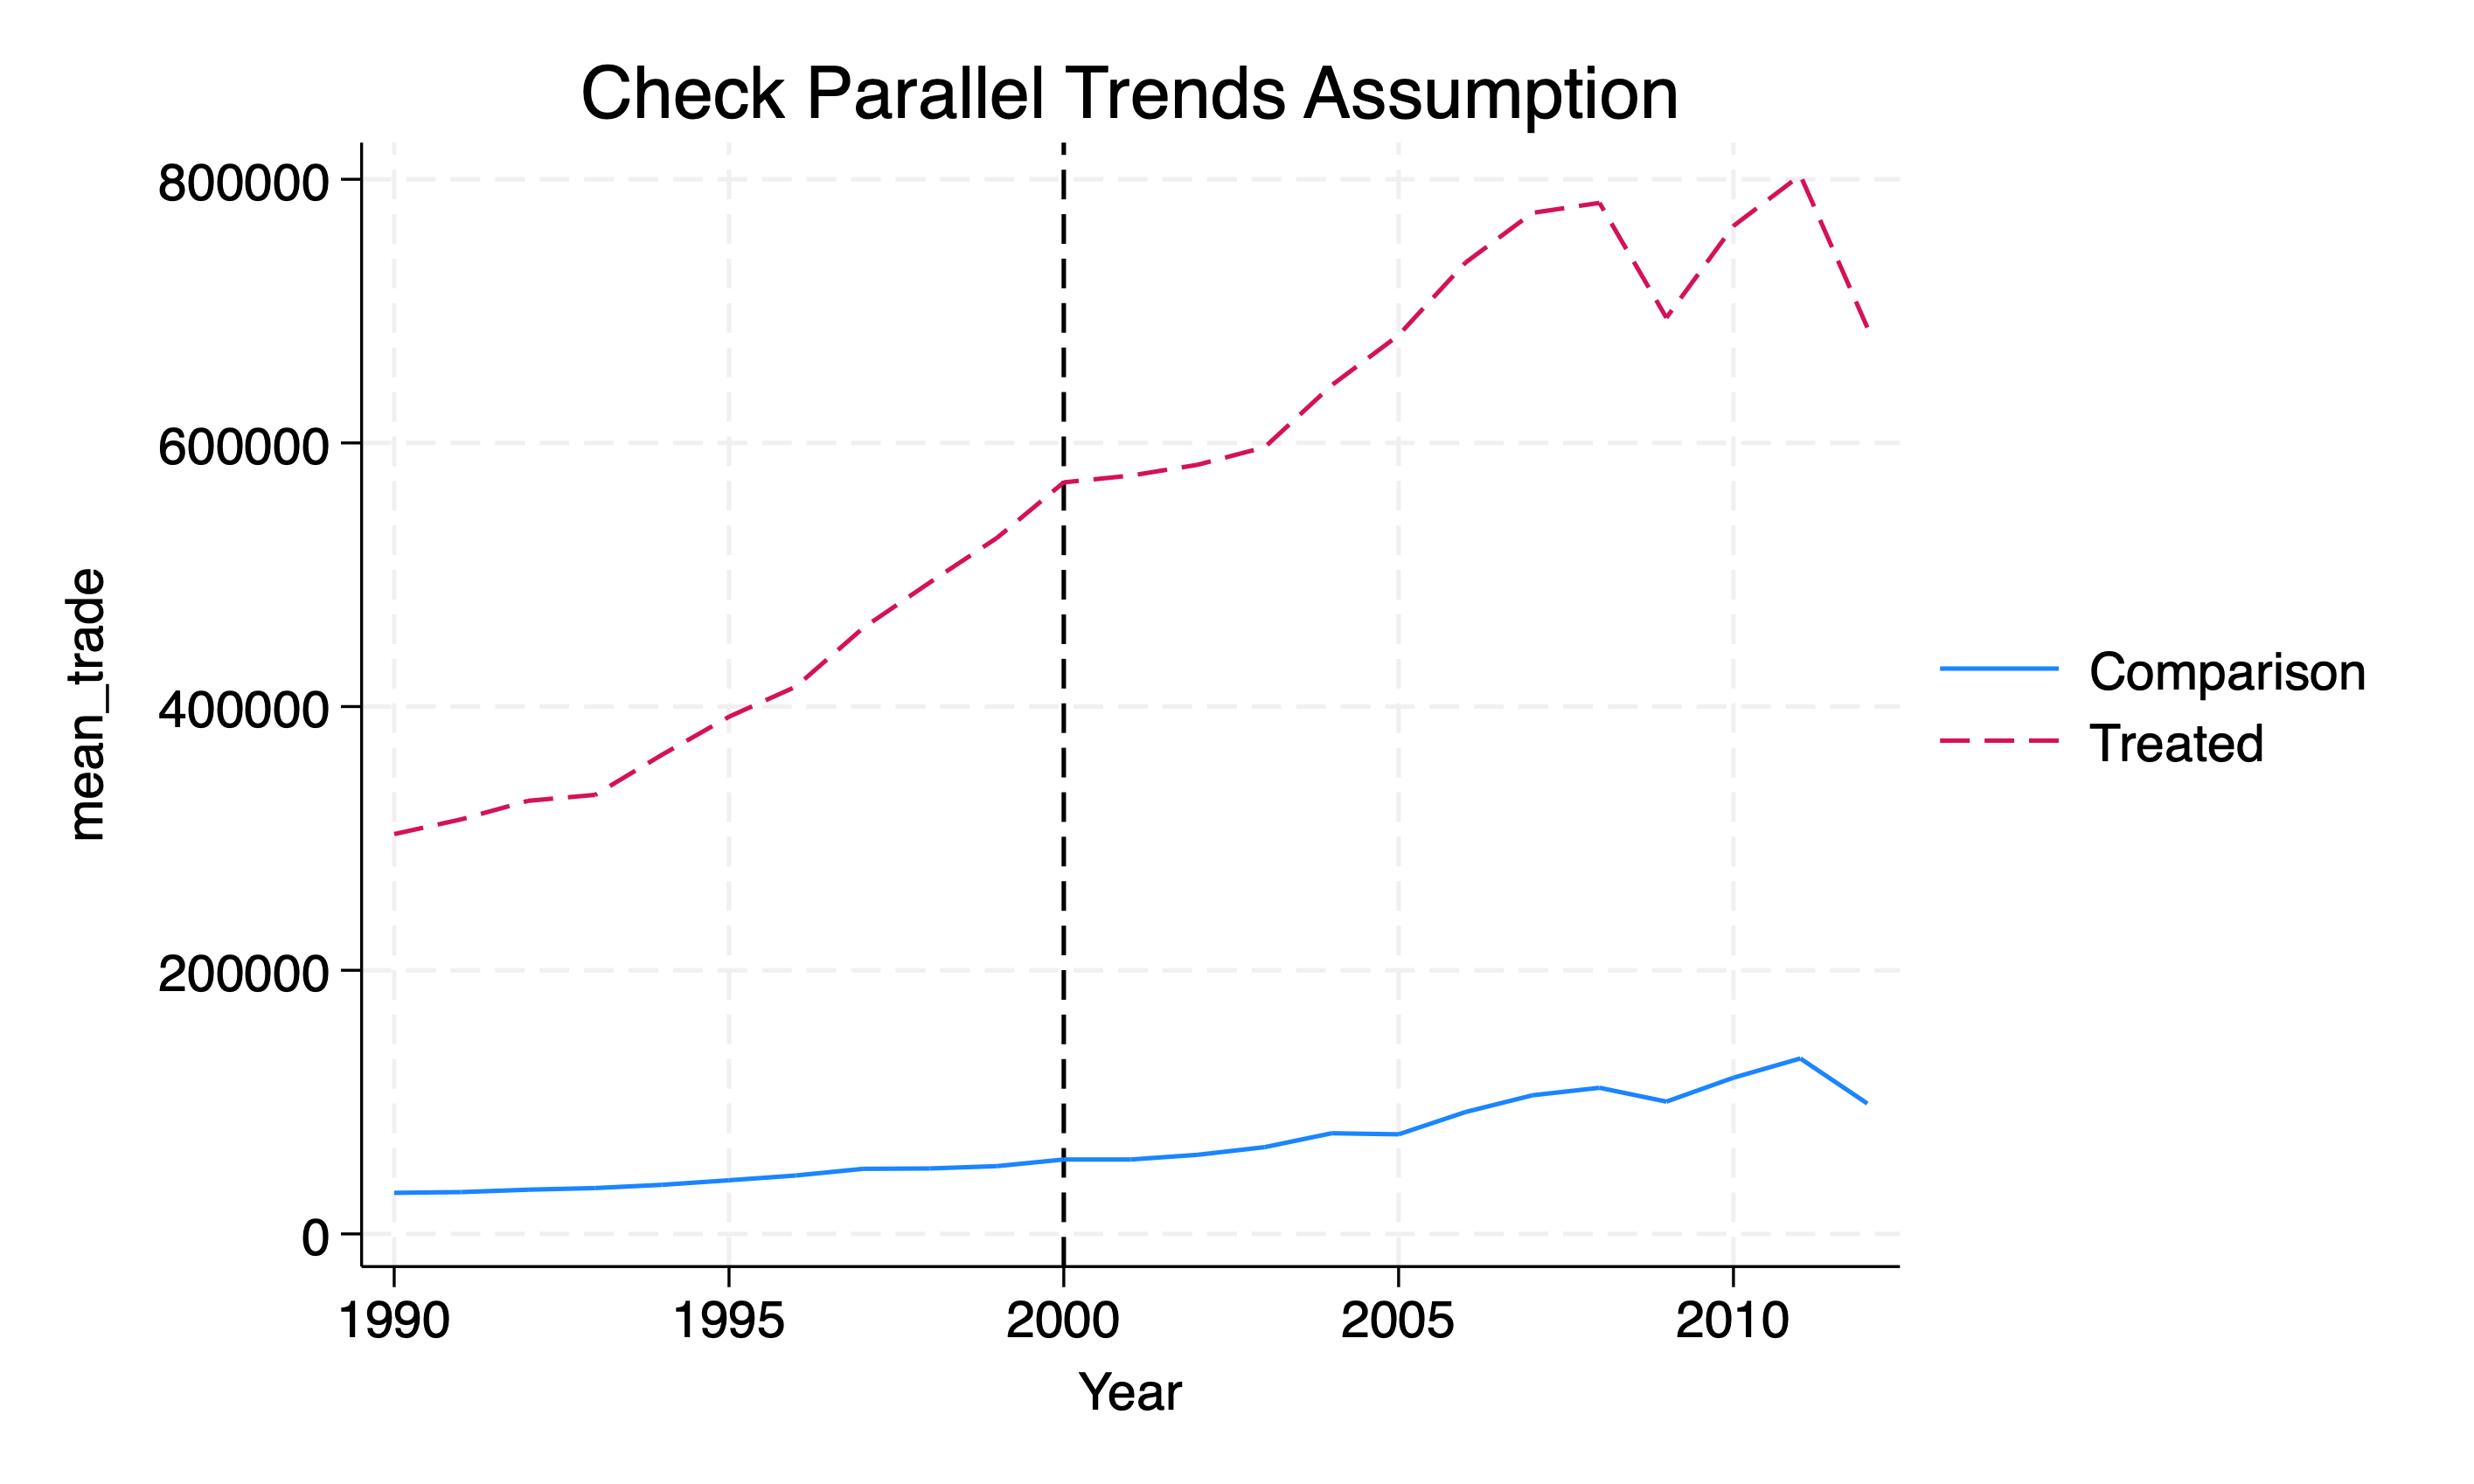
\includegraphics[keepaspectratio,alt={Inspect the Parallel Trends Assumption}]{wdi1.png}}
\caption{Inspect the Parallel Trends Assumption}
\end{figure}

\section{\texorpdfstring{\emph{xtdidregress}}{xtdidregress}}\label{xtdidregress}

We have other commands for estimating difference-in-differences, such as the \emph{xtdidregress} and \emph{didregress} commands. These commands will estimate our \(\delta^{ATET}_{DD}\) of interest.

Why should we use this command? They provide helpful post-estimation commands for testing the parallel trends assumption!

\begin{Shaded}
\begin{Highlighting}[]
\NormalTok{xtdidregress (trade) (treat\_post), }\FunctionTok{group}\NormalTok{(countrynum) time(}\FunctionTok{year}\NormalTok{)}
\end{Highlighting}
\end{Shaded}

\begin{verbatim}
Treatment and time information

Time variable: year
Control:       treat_post = 0
Treatment:     treat_post = 1
-----------------------------------
             |   Control  Treatment
-------------+---------------------
Group        |
  countrynum |       132         21
-------------+---------------------
Time         |
     Minimum |      1990       2000
     Maximum |      2006       2000
-----------------------------------

Difference-in-differences regression                     Number of obs = 2,814
Data type: Longitudinal

                           (Std. err. adjusted for 153 clusters in countrynum)
------------------------------------------------------------------------------
             |               Robust
       trade | Coefficient  std. err.      t    P>|t|     [95% conf. interval]
-------------+----------------------------------------------------------------
ATET         |
  treat_post |
   (1 vs 0)  |   254619.5   84665.83     3.01   0.003     87345.69    421893.2
------------------------------------------------------------------------------
Note: ATET estimate adjusted for panel effects and time effects.
Note: Treatment occurs at different times.
\end{verbatim}

We get the same result, such that trade increases \$254,619.5 millions or 255 billion 2005 US dollars

We can also add some covariates in case the parallel trends is conditional on controlling for covariates.

\begin{Shaded}
\begin{Highlighting}[]
\NormalTok{xtdidregress (trade unemp polity) (treat\_post), }\FunctionTok{group}\NormalTok{(countrynum) time(}\FunctionTok{year}\NormalTok{)}
\end{Highlighting}
\end{Shaded}

\begin{verbatim}
Treatment and time information

Time variable: year
Control:       treat_post = 0
Treatment:     treat_post = 1
-----------------------------------
             |   Control  Treatment
-------------+---------------------
Group        |
  countrynum |       132         21
-------------+---------------------
Time         |
     Minimum |      1990       2000
     Maximum |      2006       2000
-----------------------------------

Difference-in-differences regression                     Number of obs = 2,804
Data type: Longitudinal

                           (Std. err. adjusted for 153 clusters in countrynum)
------------------------------------------------------------------------------
             |               Robust
       trade | Coefficient  std. err.      t    P>|t|     [95% conf. interval]
-------------+----------------------------------------------------------------
ATET         |
  treat_post |
   (1 vs 0)  |   253104.1   85410.71     2.96   0.004     84358.69    421849.5
------------------------------------------------------------------------------
Note: ATET estimate adjusted for covariates, panel effects, and time effects.
Note: Treatment occurs at different times.
\end{verbatim}

Our estimate is little change after controlling for unemployment and political system of the country. Our estimate is \(\hat{\delta}^{ATET}_{DD}=\$253B\).

\chapter{Postestimation Command}\label{postestimation-command}

The question remains if our parallel trends assummption holds. We visually inspected the parallel trends assumption with a graph, but we did not test any null hypotheses. With the \emph{xtdidregress} and \emph{didregress} commands we have two helpful commands: \emph{estat ptrends} and \emph{estat trendplots}.

\section{\texorpdfstring{\emph{estat ptrends}}{estat ptrends}}\label{estat-ptrends}

Let's test the null hypothesis that the trends between treatment and comparison are the same. We will use the diff-in-diff without covariates first

\begin{Shaded}
\begin{Highlighting}[]
\KeywordTok{quietly}\NormalTok{ xtdidregress (trade) (treat\_post), }\FunctionTok{group}\NormalTok{(countrynum) time(}\FunctionTok{year}\NormalTok{)}
\KeywordTok{estat}\NormalTok{ ptrends}
\end{Highlighting}
\end{Shaded}

\begin{verbatim}
Parallel-trends test (pretreatment time period)
H0: Linear trends are parallel

F(1, 152) =   9.09
 Prob > F = 0.0030
\end{verbatim}

Our \(F\)-statistic is \(9.09\) and we reject the null hypothesis at the 1\% level. Now let's add the covariates to see if parallel trends are conditional on additional covariates of unemployment and political system.

\begin{Shaded}
\begin{Highlighting}[]
\KeywordTok{quietly}\NormalTok{ xtdidregress (trade unemp polity) (treat\_post), }\FunctionTok{group}\NormalTok{(countrynum) time(}\FunctionTok{year}\NormalTok{)}
\KeywordTok{estat}\NormalTok{ ptrends}
\end{Highlighting}
\end{Shaded}

\begin{verbatim}
Parallel-trends test (pretreatment time period)
H0: Linear trends are parallel

F(1, 152) =   8.85
 Prob > F = 0.0034
\end{verbatim}

Our \(F\)-statistic barely changes and we reject the null hypothesis at the 1\% level.

\section{\texorpdfstring{\emph{estat trendsplot}}{estat trendsplot}}\label{estat-trendsplot}

Even though we reject the null hypothesis at the 1\% level, we can still provide a visualization that is easier to implement than our \emph{twoway line} graph above. With \emph{estat trendsplot}, the syntax is more concise and less likely to have an operator error. With the \emph{twoway line} command, we need to make sure to graph both treatment and comparison lines.

We will compare the parallel trends with and without covariates. The command is the same regardless if we have covariates or not.

\begin{Shaded}
\begin{Highlighting}[]
\KeywordTok{quietly}\NormalTok{ xtdidregress (trade) (treat\_post), }\FunctionTok{group}\NormalTok{(countrynum) time(}\FunctionTok{year}\NormalTok{)}
\KeywordTok{estat}\NormalTok{ trendplots, }\BaseNTok{ytitle}\NormalTok{(Trade }\KeywordTok{in}\NormalTok{ millions }\KeywordTok{of}\NormalTok{ 2005 USD) }\KeywordTok{xlabel}\NormalTok{(1990(2)2012)}
\end{Highlighting}
\end{Shaded}

\begin{figure}
\centering
\pandocbounded{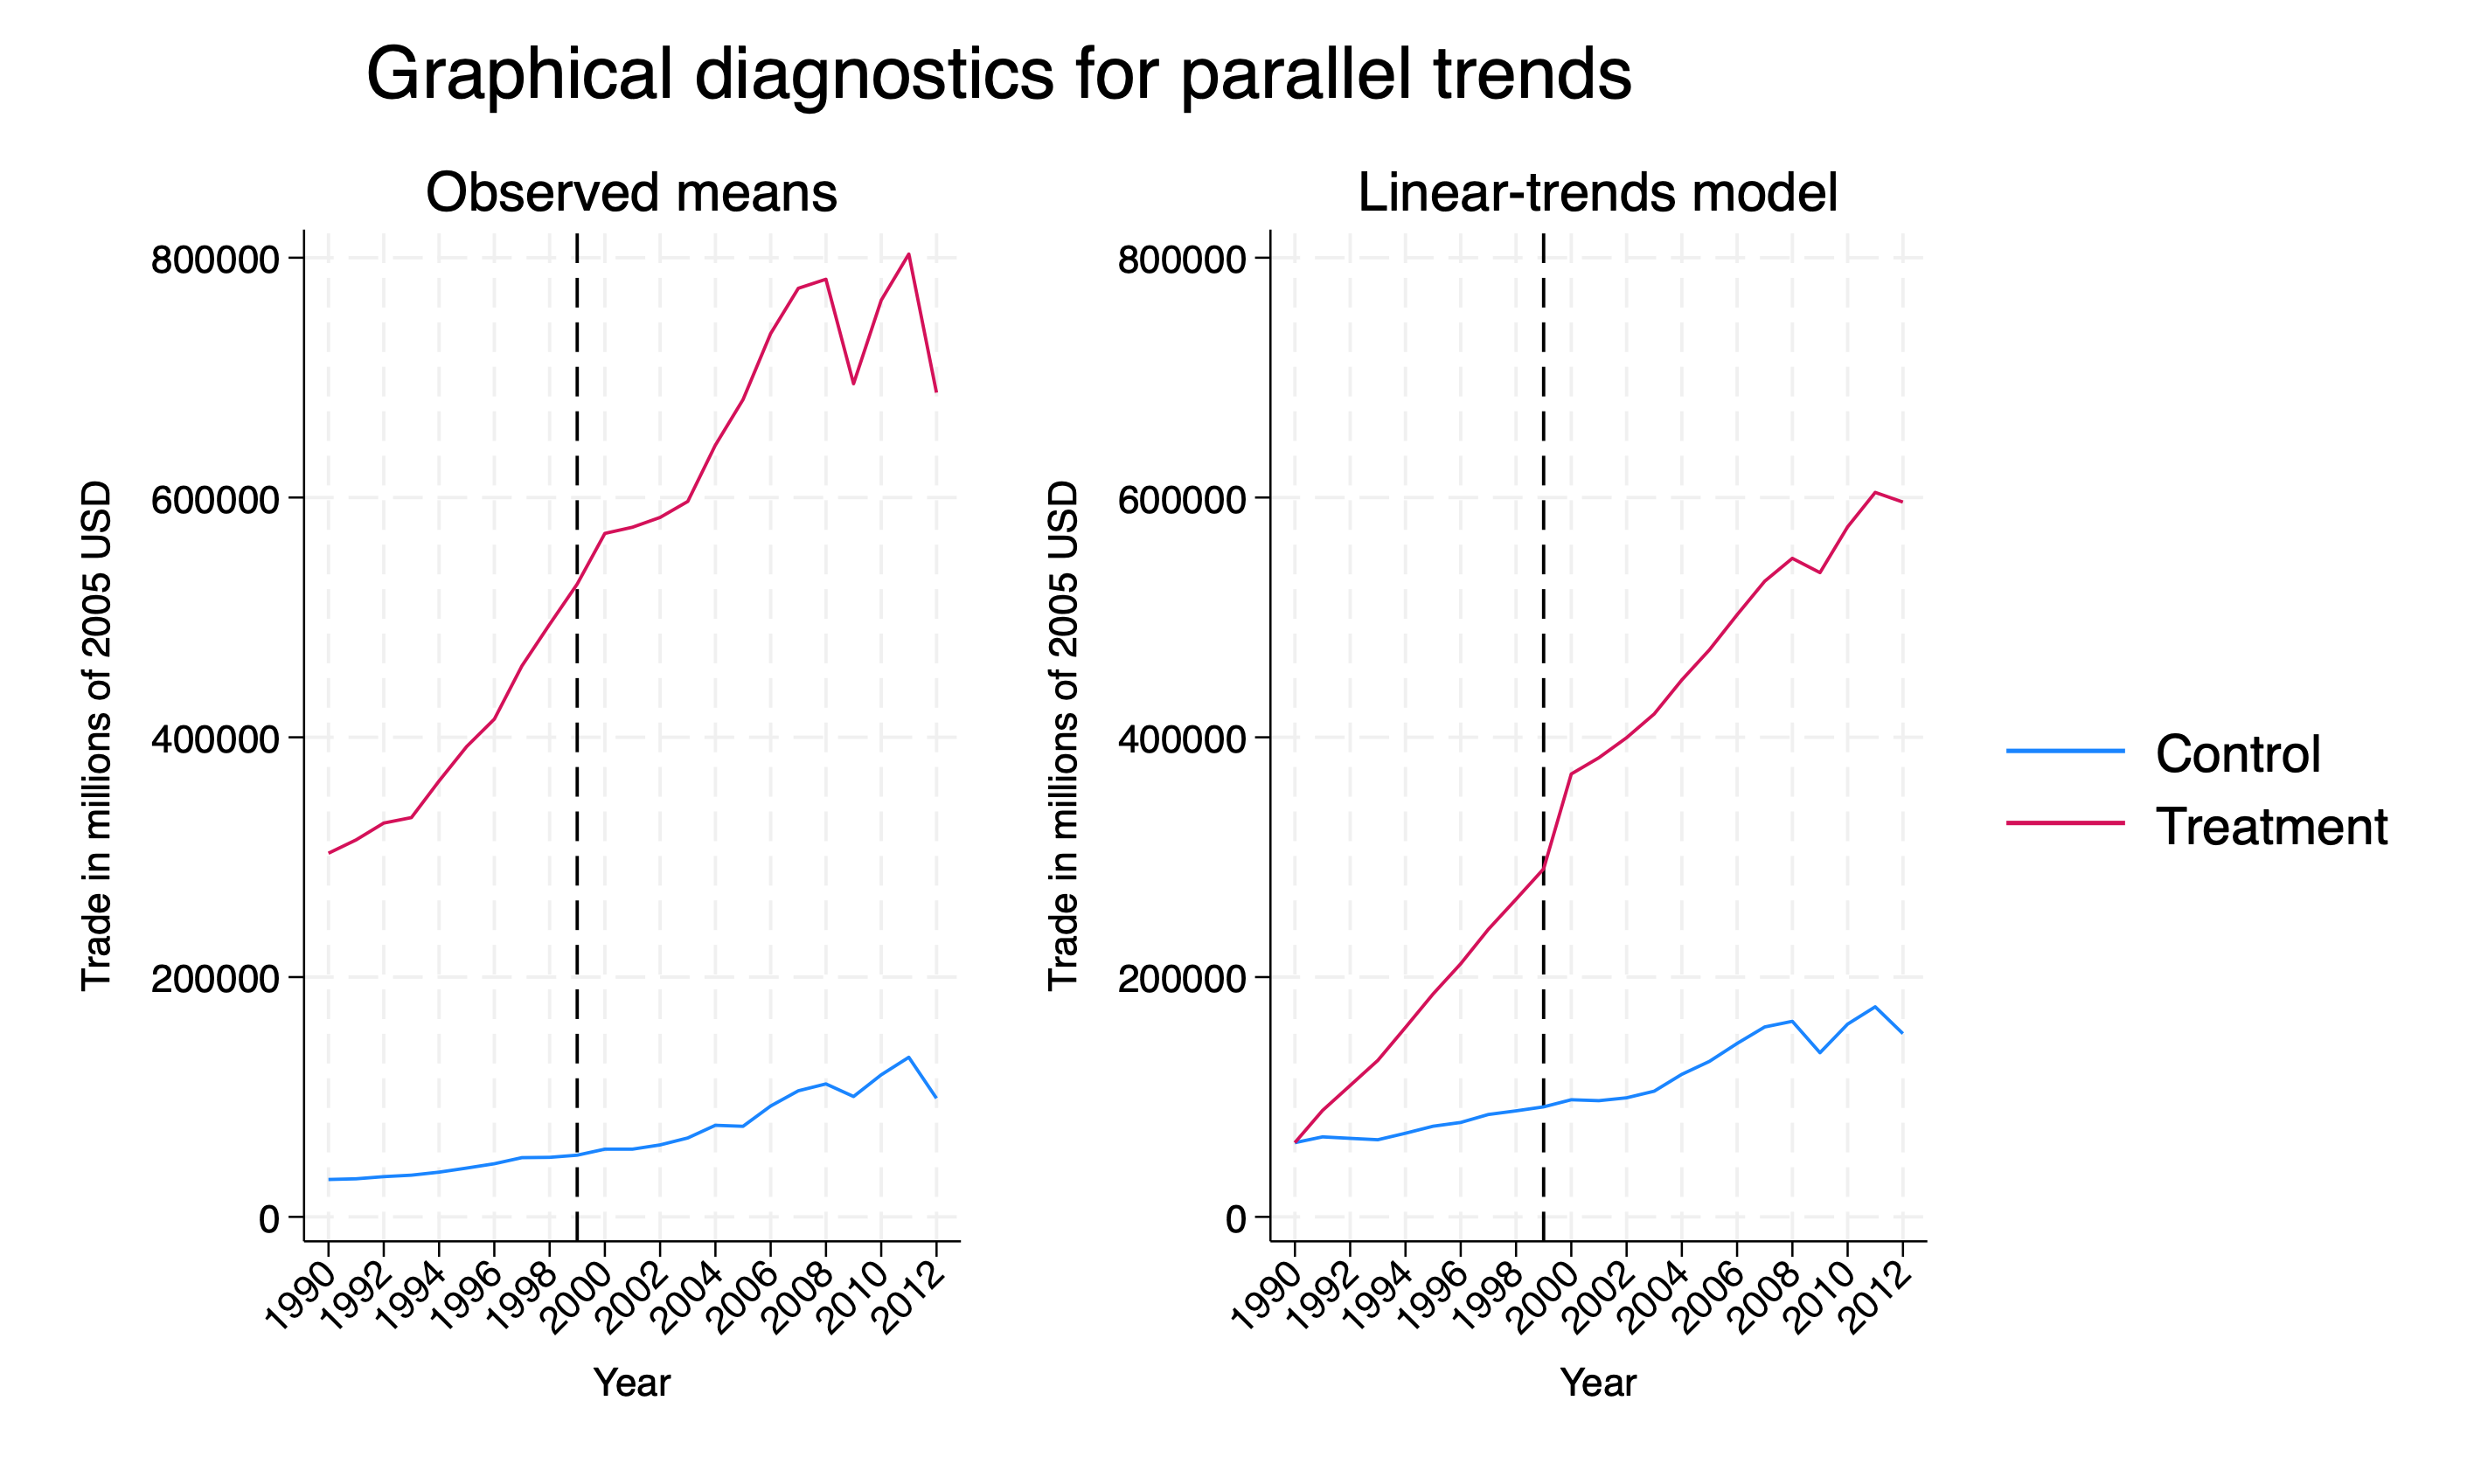
\includegraphics[keepaspectratio,alt={Parallel trends without covariates}]{ptrend1.png}}
\caption{Parallel trends without covariates}
\end{figure}

We can clearly see that the parallel trend assumption does not hold. This visually confirms what we saw with out \(F\)-test.

Next, we will add covariates.

\begin{Shaded}
\begin{Highlighting}[]
\KeywordTok{quietly}\NormalTok{ xtdidregress (trade) (treat\_post), }\FunctionTok{group}\NormalTok{(countrynum) time(}\FunctionTok{year}\NormalTok{)}
\KeywordTok{estat}\NormalTok{ trendplots, }\BaseNTok{ytitle}\NormalTok{(Trade }\KeywordTok{in}\NormalTok{ millions }\KeywordTok{of}\NormalTok{ 2005 USD) }\KeywordTok{xlabel}\NormalTok{(1990(2)2012)}
\end{Highlighting}
\end{Shaded}

\begin{figure}
\centering
\pandocbounded{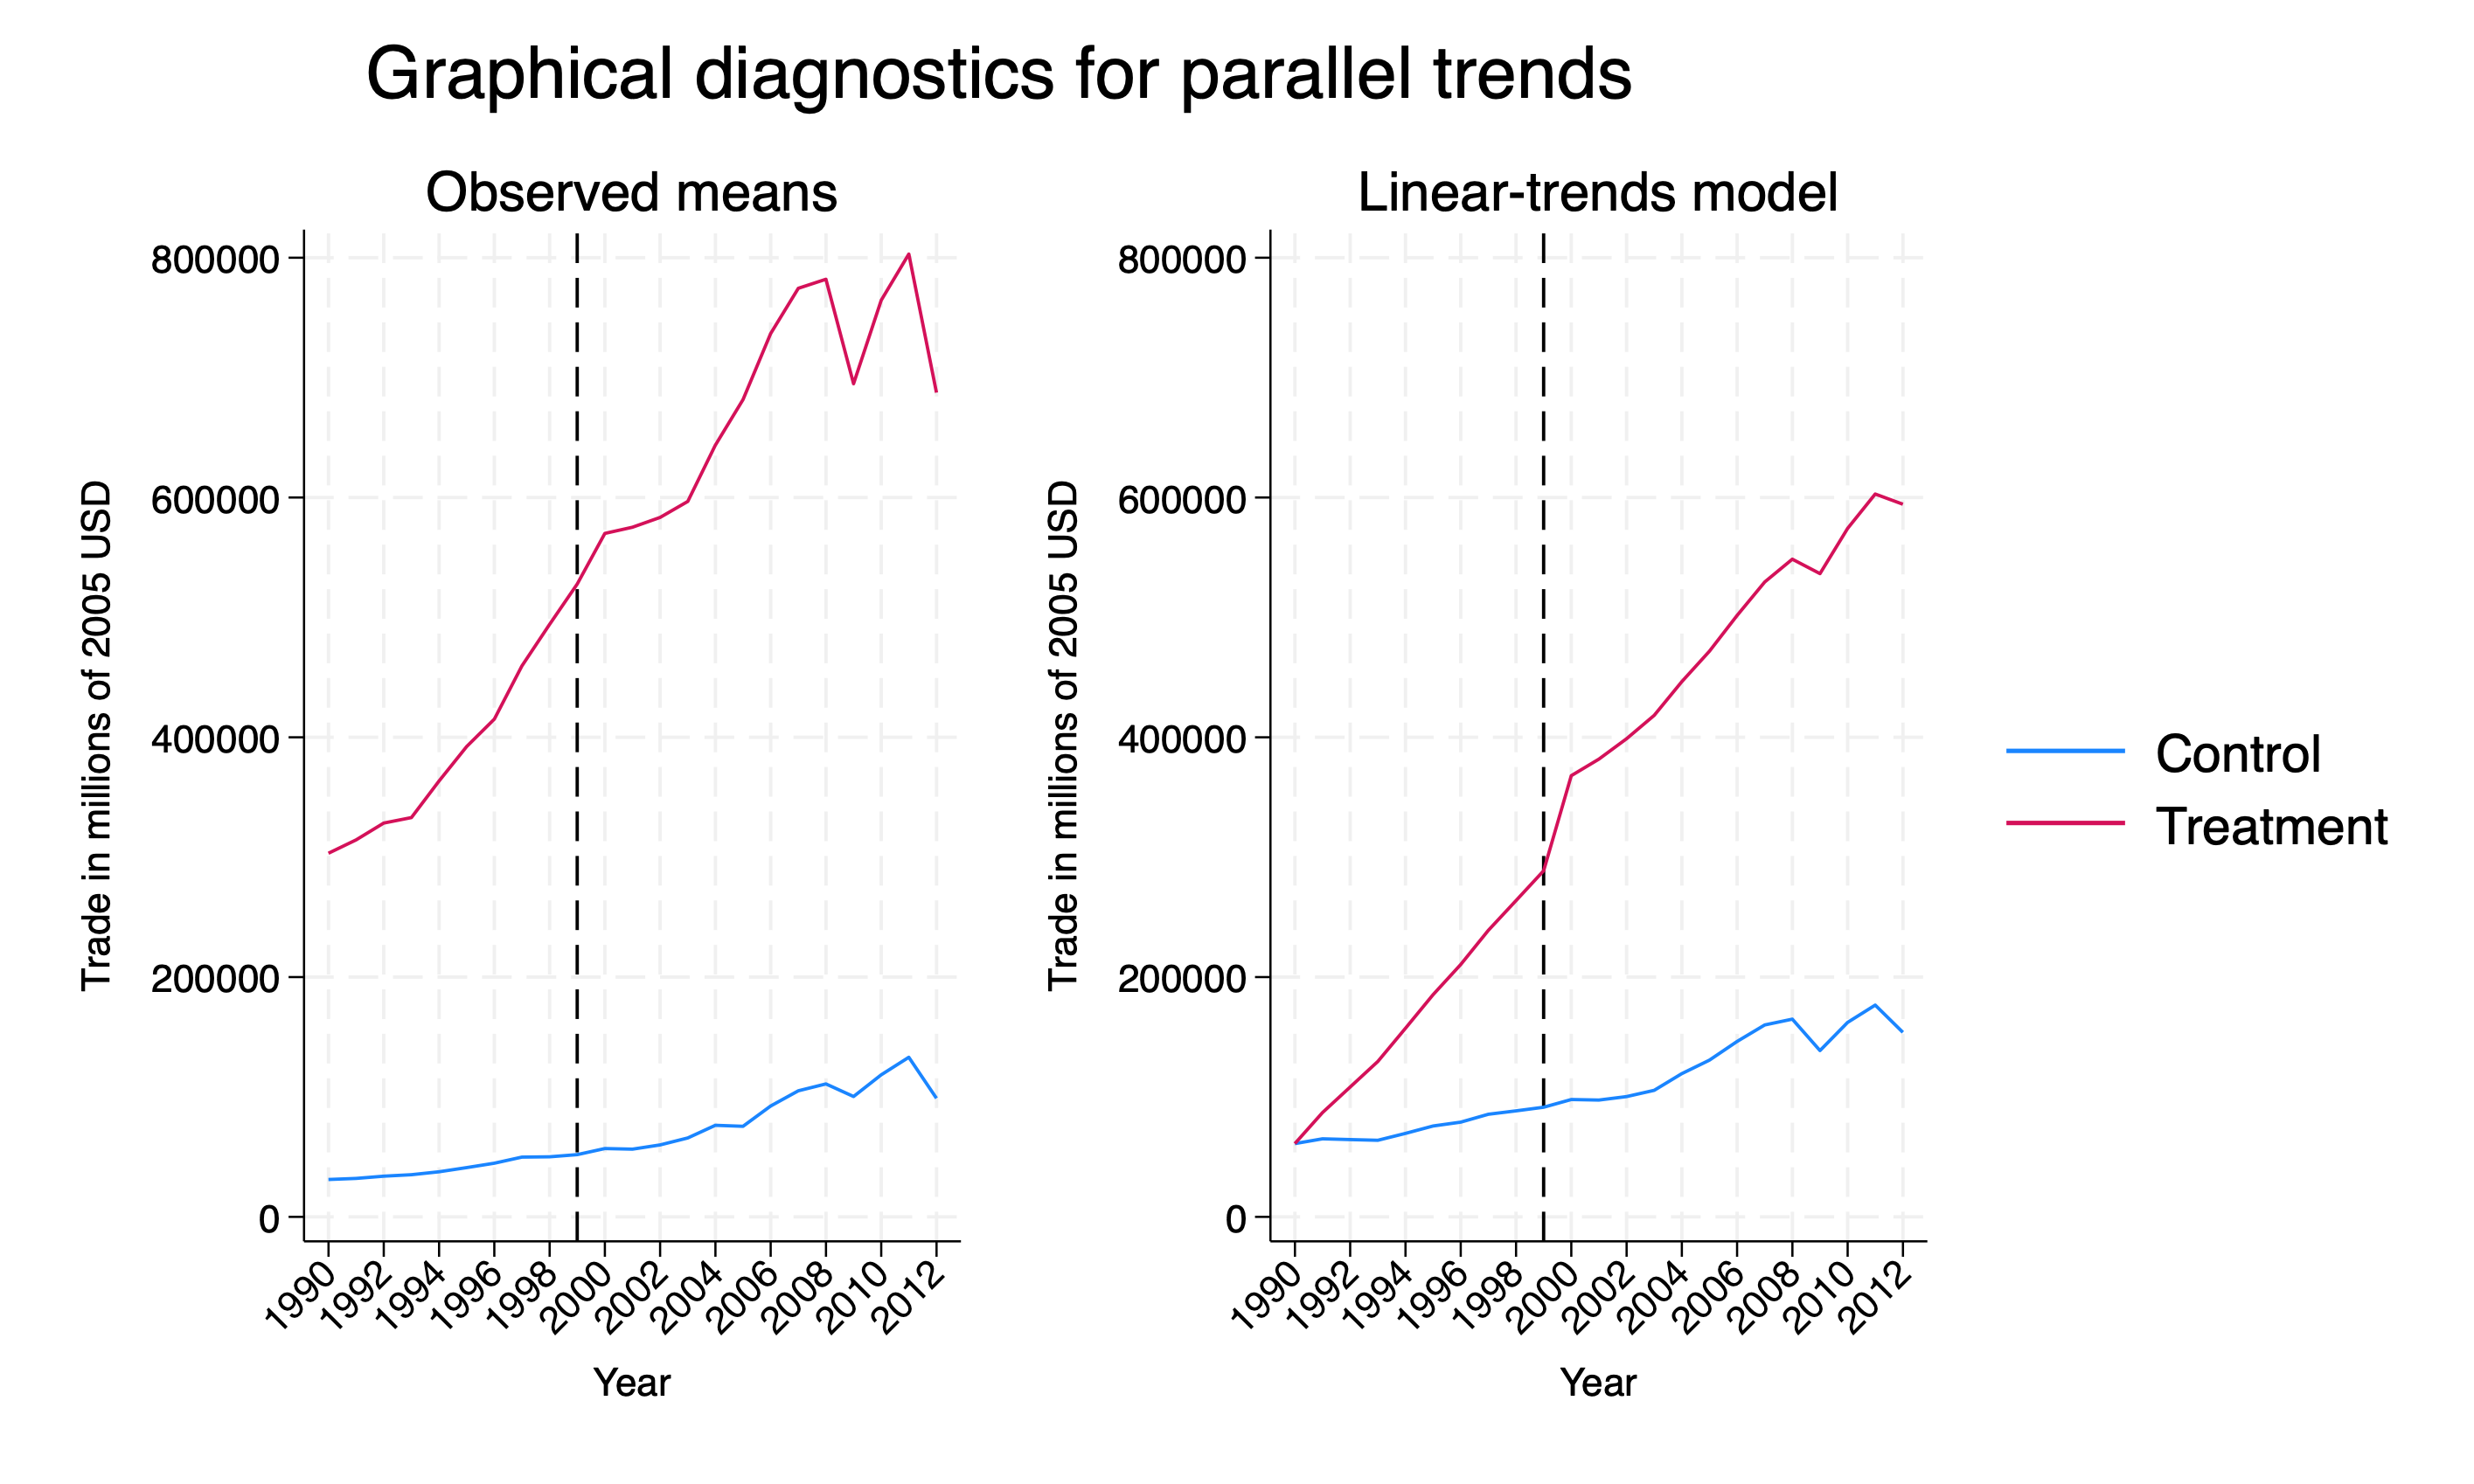
\includegraphics[keepaspectratio,alt={Parallel trends with covariates}]{ptrend2.png}}
\caption{Parallel trends with covariates}
\end{figure}

Again, we clearly see that the parallel trends assumption does not hold even if we add covariates.

\chapter{Placebo Tests: False Timing}\label{placebo-tests-false-timing}

Our second major type of placebo test for difference-in-differences estimator is false timing. We can accomplish this by changing our \(t\) to \(t-n\).

\section{False Timing}\label{false-timing}

For our trade example, our treatment date is the year 2000, but let's set the date to 1995.

\begin{Shaded}
\begin{Highlighting}[]
\KeywordTok{gen}\NormalTok{ post2 = .}
\KeywordTok{replace}\NormalTok{ post2 = 0 }\KeywordTok{if} \FunctionTok{year}\NormalTok{ \textless{} 1995}
\KeywordTok{replace}\NormalTok{ post2 = 1 }\KeywordTok{if} \FunctionTok{year}\NormalTok{ \textgreater{}= 1995}

\KeywordTok{gen}\NormalTok{ treat\_post2=treatment*post2}
\end{Highlighting}
\end{Shaded}

We should expect no statistically significant difference between treatment and comparison for our placebo test.

\begin{Shaded}
\begin{Highlighting}[]
\NormalTok{xtdidregress (trade) (treat\_post2), }\FunctionTok{group}\NormalTok{(countrynum) time(}\FunctionTok{year}\NormalTok{)}
\end{Highlighting}
\end{Shaded}

\begin{verbatim}
Treatment and time information

Time variable: year
Control:       treat_post2 = 0
Treatment:     treat_post2 = 1
-----------------------------------
             |   Control  Treatment
-------------+---------------------
Group        |
  countrynum |       132         21
-------------+---------------------
Time         |
     Minimum |      1990       1995
     Maximum |      2006       2000
-----------------------------------

Difference-in-differences regression                     Number of obs = 2,814
Data type: Longitudinal

                           (Std. err. adjusted for 153 clusters in countrynum)
------------------------------------------------------------------------------
             |               Robust
       trade | Coefficient  std. err.      t    P>|t|     [95% conf. interval]
-------------+----------------------------------------------------------------
ATET         |
 treat_post2 |
   (1 vs 0)  |     253834   83426.64     3.04   0.003     89008.47    418659.5
------------------------------------------------------------------------------
Note: ATET estimate adjusted for panel effects and time effects.
Note: Treatment occurs at different times.
\end{verbatim}

We reject the null hypothesis that the parameter is equal to zero, so our placebo test fails. There is something going on with these countries that may increase trade relative to other countries besides the trade policy change.

Cunningham, S. (2021). \emph{Causal Inference: The Mixtape}. Yale University Press.

Huber, M. (2023). \emph{Causal Analysis: Impact Evaluation and Causal Machine Learning with Applications in R}. The MIT Press.

Huntington-Klein, N. (2022). \emph{The Effect: An Introduction to Research Design and Causality}. CRC Press.

Princeton (2026). \emph{Difference-in-Differences in Stata: A step-by-step guide.} \url{https://libguides.princeton.edu/stata-did/1\#s-lg-box-wrapper-41689126}

\bibliography{book.bib,packages.bib}

\end{document}
